\chapter{Joint Retrieval of Ozone, Pressure and Temperature}
\label{ch:FullBay}

Here we extend the hierarchical Bayesian model set up in Sec. \ref{sec:BayModelO3} to include pressure and temperature related hyper-parameters and elaborate on some aspects of prior modelling.
The MTC scheme is applied to jointly provide posterior distributions of ozone, pressure and temperature.
Additionally, the reader is guided through the process of setting up an efficient TT approximation of the higher-dimensional marginal posterior.



\section{Hierarchical Bayesian Framework}
\label{sec:FullHierarch}
\begin{figure}[thb!]
	\centering
	\begin{tikzpicture}
		\node[roundnode2] at (-4.5,6.5) (Q)     {$\bm{Q}$};
		\node[roundnode2] at (-3,5) (x)     {$\bm{x}$};
		\node[align=center] at (-1,3.75) (A)    {$\bm{A}_{\bm{\theta}} \coloneqq \bm{M}\bm{A}_L(p_0,b,T_0,\bm{h_T},\bm{a})$};
		\node[roundnode2] at (-1,2.5) (u)    {$\Omega$};
		\node[rectnode] at (-1,1) (y)    {$\bm{y}$};
		\node[roundnode2] at (-3,2.5) (e)    {$\bm{\eta}$};
		\node[roundnode2] at (-7.5,6.5) (S)    {$\bm{\Sigma}$};
		\node[roundnode2] at (-8.5,8) (s)    {$\gamma$};
		\node[roundnode2] at (-6,8) (d)    {$\delta$};
		\node[roundnode2] at (3,6.5) (t)     {$\bm{T}$};
		\node[roundnode2] at (-1,6.5) (p)     {$\bm{p}$};
		\node[roundnode2] at (1,5) (pt)     {$\bm{p}/\bm{T}$};
		\node[roundnode2] at (0,8) (b1)    {$b$};
		%\node[roundnode2] at (1,8) (b2)    {$b_2$};
		%\node[roundnode2] at (-2,8) (h1)    {$h_{0}$};
		\node[roundnode2] at (-1.5,8) (p0)    {$p_0$};
		\node[roundnode2] at (2.25,8) (ht)    {$\bm{h_T}$};
		\node[roundnode2] at (3.25,8) (ct)    {$T_0$};
		\node[roundnode2] at (4.25,8) (at)    {$\bm{a}$};
		
		\node[roundnode2] at (0,10) (b1hyp)    {$\bm{\theta}_{b}$};
		%\node[roundnode2] at (-2.5,10) (h1hyp)    {$\bm{\theta}_{h_{0}}$};
		\node[roundnode2] at (-1.5,10) (p0hyp)    {$\bm{\theta}_{p_{0}}$};
		\node[roundnode2] at (2,10) (hthyp)    {$\bm{\theta}_{\bm{h}_T}$};
		\node[roundnode2] at (3.25,10) (cthyp)    {$\bm{\theta}_{T_{0}}$};
		\node[roundnode2] at (4.5,10) (athyp)    {$\bm{\theta}_{\bm{a}}$};
		
		\node[roundnode2] at (-8.5,10) (shyp)    {$\bm{\theta}_{\gamma}$};
		\node[roundnode2] at (-6,10) (dhyp)    {$\bm{\theta}_{\delta}$};
		
		%Lines
		
		
		\draw[->, very thick] (S) -- (e);
		\draw[->, mydotted, very thick] (s) -- (S);
		\draw[->, very thick] (u) -- (y);
		\draw[->, mydotted, very thick] (A) -- (u);
		\draw[->, mydotted,  very thick] (x) -- (A);
		\draw[->, mydotted, very thick] (p) -- (pt);
		\draw[->, mydotted, very thick] (t) -- (pt);
		\draw[->, mydotted, very thick] (pt) -- (A);
		%\draw[->, mydotted, very thick] (h1) -- (p);
		\draw[->, mydotted, very thick] (p0) -- (p);
		\draw[->, mydotted, very thick] (b1) -- (p); 
		%\draw[->, very thick] (b2.south) -- (p.east); 
		\draw[->, mydotted, very thick] (d) -- (Q); 
		\draw[->, mydotted, very thick] (e) -- (y); 
		
		\draw[->, very thick] (Q.south east) -- (x.north west); 
		\draw[->, mydotted, very thick] (ht.south) -- (t.north west);
		\draw[->, mydotted, very thick] (ct.south) -- (t.north);
		\draw[->, mydotted, very thick] (at.south) -- (t.north east);
		
		
		\draw[->, very thick] (b1hyp) -- (b1);
		%\draw[->, very thick] (h1hyp) -- (h1);
		\draw[->, very thick] (p0hyp) -- (p0);
		\draw[->, very thick] (hthyp) -- (ht);
		\draw[->, very thick] (cthyp) -- (ct);
		\draw[->, very thick] (athyp) -- (at);
		\draw[->, very thick] (shyp) -- (s);
		\draw[->, very thick] (dhyp) -- (d);
		
		\node[fit=(s)(at),draw,dotted,black, rounded corners] {};
		\node[align =center] at (-3.75,8) (T1) {hyper-parameters};
		\node[align =center] at (-4.5,5) (T2) {parameter};
		\node[fit=(x)(T2),draw,dotted,black, rounded corners] {};
		
	\end{tikzpicture} 
	\caption[Directed acyclic graph of Bayesian model for ozone $\bm{x}$, pressure $\bm{p}$ and temperature $\bm{T}$.]{DAG of the hierarchical Bayesian model including ozone $\bm{x}$, pressure $\bm{p}$ and temperature $\bm{T}$. The hyper-parameters $\bm{h}_T= \{ h_{T,1}, h_{T,2},h_{T,3},h_{T,4},h_{T,5},h_{T,6}\}$, $\bm{a} = \{ a_0, a_1, a_2,a_3,a_4,a_5,a_6\}$, $T_0$, $b$ and $p_0$ deterministically (dotted line) describe pressure through Eq.~\ref{eq:pressFunc} and temperature through Eq.~\ref{eq:tempFunc}. In this case, the hyper-parameters $\pi(p_0,b,T_0,\bm{h_T},\bm{a})$ are a normally distributed a-priori. That is why $\bm{\theta}_{\bm{h}_T},\bm{\theta}_{\bm{a}}, \bm{\theta}_{T_{0}},\bm{\theta}_{b} , \bm{\theta}_{p_0}$ represent means and STDs e.g.,~$b \sim \mathcal{N}(\mu_b, \sigma^2_b)$ and $\bm{\theta}_{b} = \{\mu_b, \sigma_b\}$.
	As previously described in Sec.~\ref{sec:BayModelO3}, $\bm{\theta}_{\gamma}, \bm{\theta}_{\delta}$ determine gamma distributions e.g., $\gamma \sim \Gamma(\alpha_{\gamma},\beta_{\gamma}) $ with $\bm{\theta}_{\gamma} = 	\{\alpha_{\gamma},\beta_{\gamma} \}$.
	The ozone parameter $\bm{x}$ is statistically (solid line) described by the prior distribution $\bm{x}| \delta \sim \mathcal{N}(0,(\delta \bm{L})^{-1}) $. 
	Here, the hyper-parameter $\delta$ accounts for smoothness in the ozone profile and defines the precision matrix $\bm{Q} = \delta \bm{L}$ as in Eq.~\ref{eq:GLapl}.
	The approximated forward model $\bm{A}_{\bm{\theta}} \coloneqq \bm{M}\bm{A}_L(p_0,b,T_0,\bm{h_T},\bm{a})$ with $\bm{\theta}  \coloneqq \{p_0, b, T_0,\bm{h}_T,\bm{a} \}$ maps the parameter and hyper-parameters to a space of all measurables $\Omega$. 
	From that space, a data set $\bm{y}$ including some additive random noise $\bm{\eta}$ is observed (square box).
	The noise covariance $\bm{\Sigma} = \gamma^{-1} \bm{I}$ of the random noise vector $\bm{\eta} \sim \mathcal{N}(0,\gamma^{-1} \bm{I} ) $ is defined by the hyper-parameter $\gamma$.}
	%Given the data we like to determine the marginal posterior distribution over the hyper-parameters $\pi(\bm{\theta}, \delta, \gamma | \bm{y})$ first and then the conditional posterior distribution for ozone $\pi(\bm{x}|\bm{\theta}, \delta, \gamma, \bm{y})$, utilising the MTC scheme.}
	\label{fig:DAGComplete}
\end{figure}
As in Sec.~\ref{sec:BayModelO3}, the DAG in Fig.~\ref{fig:DAGComplete} visualises the measurement process and conditional dependencies between the parameter and the hyper-parameters.
This hierarchical Bayesian framework includes the hyper-parameters $p_0, b$ for pressure (see Eq.~\ref{eq:pressFunc}), $\bm{a}, \bm{h}_T, T_0$ for temperature (see Eq.~\ref{eq:tempFunc}), $\delta$ for ozone smoothness and $\gamma$ for noise precision.
The hyper-parameters are described by the hyper-prior distribution $\pi(p_0,b,T_0,\bm{h_T},\bm{a}, \delta,\gamma)$ (see Sec.~\ref{subsec:PriorFull}).
Through their respective prior distributions, pressure $\bm{p}$, temperature $\bm{T}$ and ozone $\bm{x}$ progress deterministically (dashed line) into the forward model via $\bm{x} \times \bm{p} / \bm{T}$ and generate a space of all possible noise-free data $\Omega$.
Note that other variables in the RTE, such as the internal partition function and the black body radiation, are dependent on temperature (see Sec.~\ref{sec:RTE}).
From $\Omega$ we observe (square box) some data with additive normally distributed noise $\bm{\eta}$.
For brevity, we define the linear forward model matrix as
\begin{align}
	\bm{A}_{\bm{\theta}} \coloneqq \bm{M}\bm{A}_L(p_0,b,T_0,\bm{h_T},\bm{a}) 
\end{align}
with $\bm{\theta}  \coloneqq \{p_0,b,T_0,\bm{h_T},\bm{a}  \}$ accounting for the all pressure and temperature related hyper-parameters and $\bm{M}$ the affine approximation from the previous Chapter.

\clearpage
\noindent
The distributions of the hierarchical Bayesian framework are:
\begin{subequations}
	\label{eq:BayMode}
	\begin{align}
		\bm{y} |  \bm{x},\bm{\theta},\delta,\gamma  &\sim \mathcal{N}(\bm{A}_{\bm{\theta}}  \bm{x}, \gamma^{-1} \bm{I}) \label{eq:likelihoodFull} \\
		\bm{x}| \delta  &\sim \mathcal{N}(\bm{0}, (\delta \bm{L})^{-1} ) \label{eq:priorXFull} \\
		\delta  &\sim \Gamma(\alpha_{\delta} , \beta_{\delta} )\label{eq:priorDelFull} \\
		\gamma  &\sim \Gamma(\alpha_{\gamma}, \beta_{\gamma})\label{eq:priorGamFull} \\
		\bm{a}  &\sim \mathcal{N}(\bm{\mu}_{\bm{a}}, \bm{\Sigma}_{\bm{a}})\\
		\bm{h}_{\bm{T}}  &\sim \mathcal{N}(\bm{\mu}_{T}, \bm{\Sigma}_{\bm{h}_T}) \\
		T_0  &\sim \mathcal{N}(\mu_{T_0}, \sigma^2_{T_0} )\\
		p_0  &\sim \mathcal{N}(\mu_{p_0}, \sigma^2_{p_0} )\\
		b  &\sim \mathcal{N}(\mu_b, \sigma^2_b )  \label{eq:lastprior}  \, .
	\end{align}
\end{subequations}
Due to Gaussian noise $\pi(\bm{y} |  \bm{x},\bm{\theta},\delta,\gamma )$ is a normally distributed likelihood function and Eq.~\ref{eq:priorXFull} to Eq.~\ref{eq:lastprior} denote prior distributions.
Before formulating the posterior distribution, we carefully define $\bm{\theta}_{\gamma}, \bm{\theta}_{\delta},\bm{\theta}_{p_0},\bm{\theta}_{b},\bm{\theta}_{\bm{h}},\bm{\theta}_{T_0},\bm{\theta}_{\bm{a}}$, the hyper-prior scales, shapes, means and variances, which are explicitly given in Tab.~\ref{tab:priors}.

\subsection{Prior Modelling}
\label{subsec:PriorFull}
\begin{figure}[ht!]
	\centering
	\input{TrueTemp.pdf_tex}
	%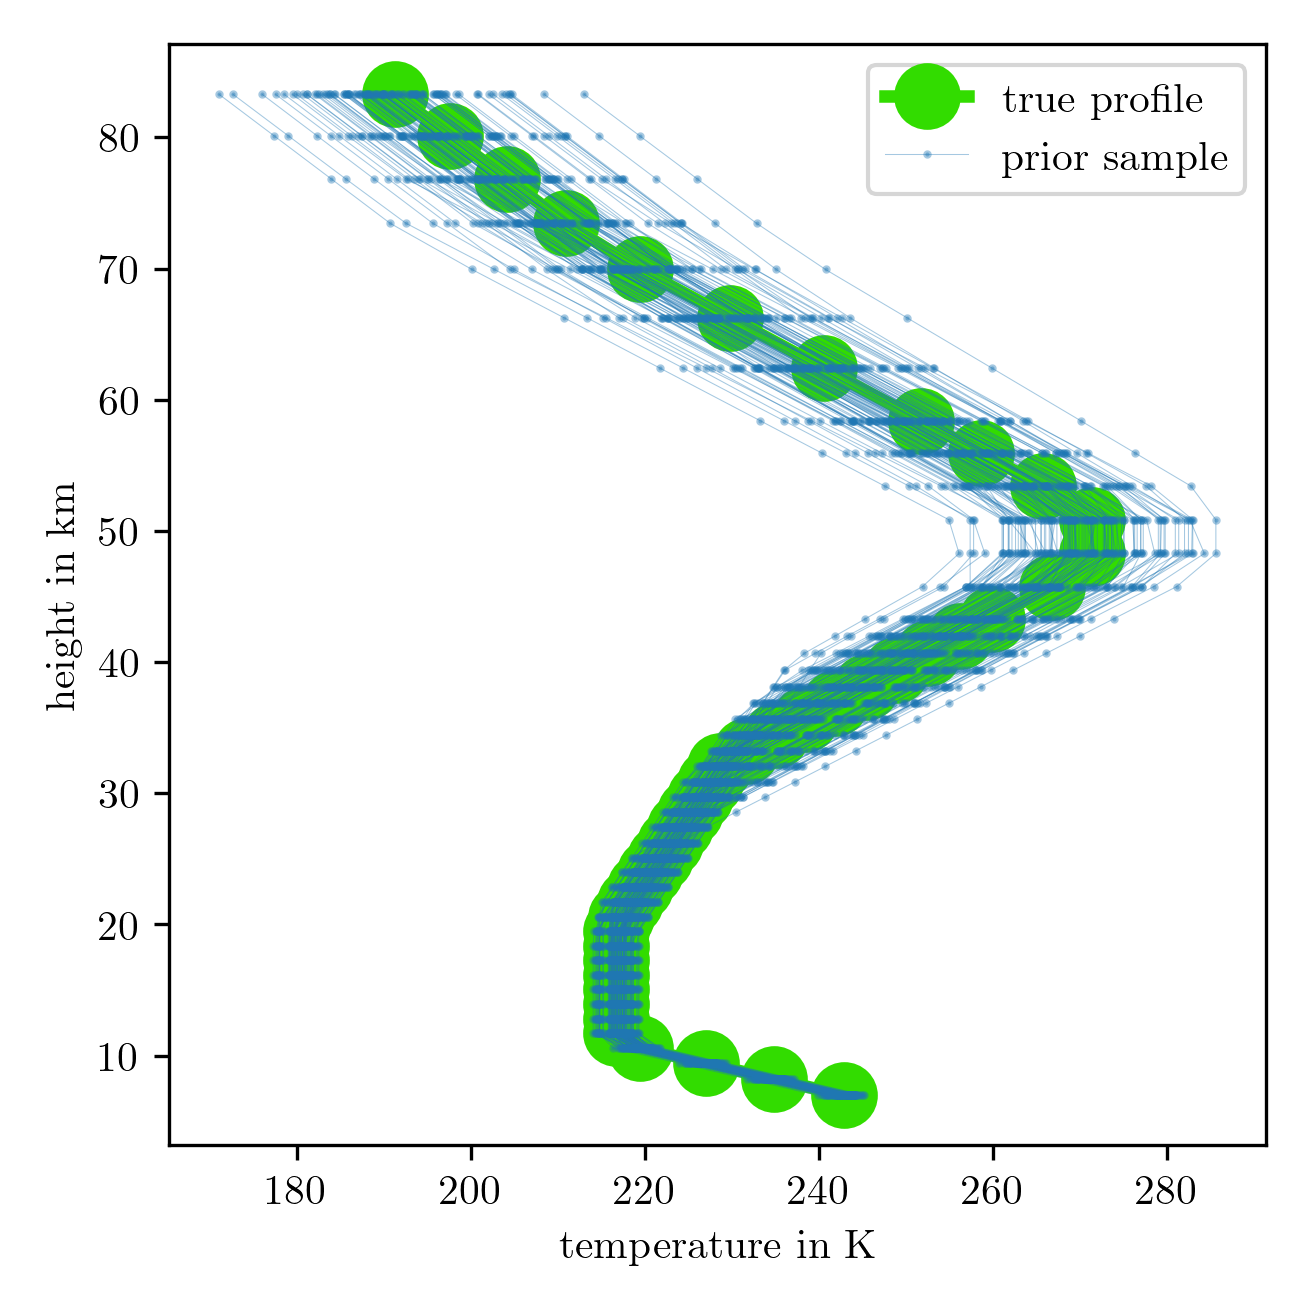
\includegraphics{PriorTempPostMeanSigm.png}
	\caption[Prior Samples of $\bm{T}$ according to the respective hyper-prior distribution.]{Prior samples from the hyper-prior distribution of $\bm{h}_T$, $\bm{a}$ and $T_0$, as defined in Tab.~\ref{tab:priors}, where we calculate $\bm{T}$ according to the function in Eq.~\ref{eq:tempFunc}.}
	\label{fig:PriorTemp}
\end{figure}
\begin{figure}[ht!]
	\centering
	\input{TruePress.pdf_tex}
	%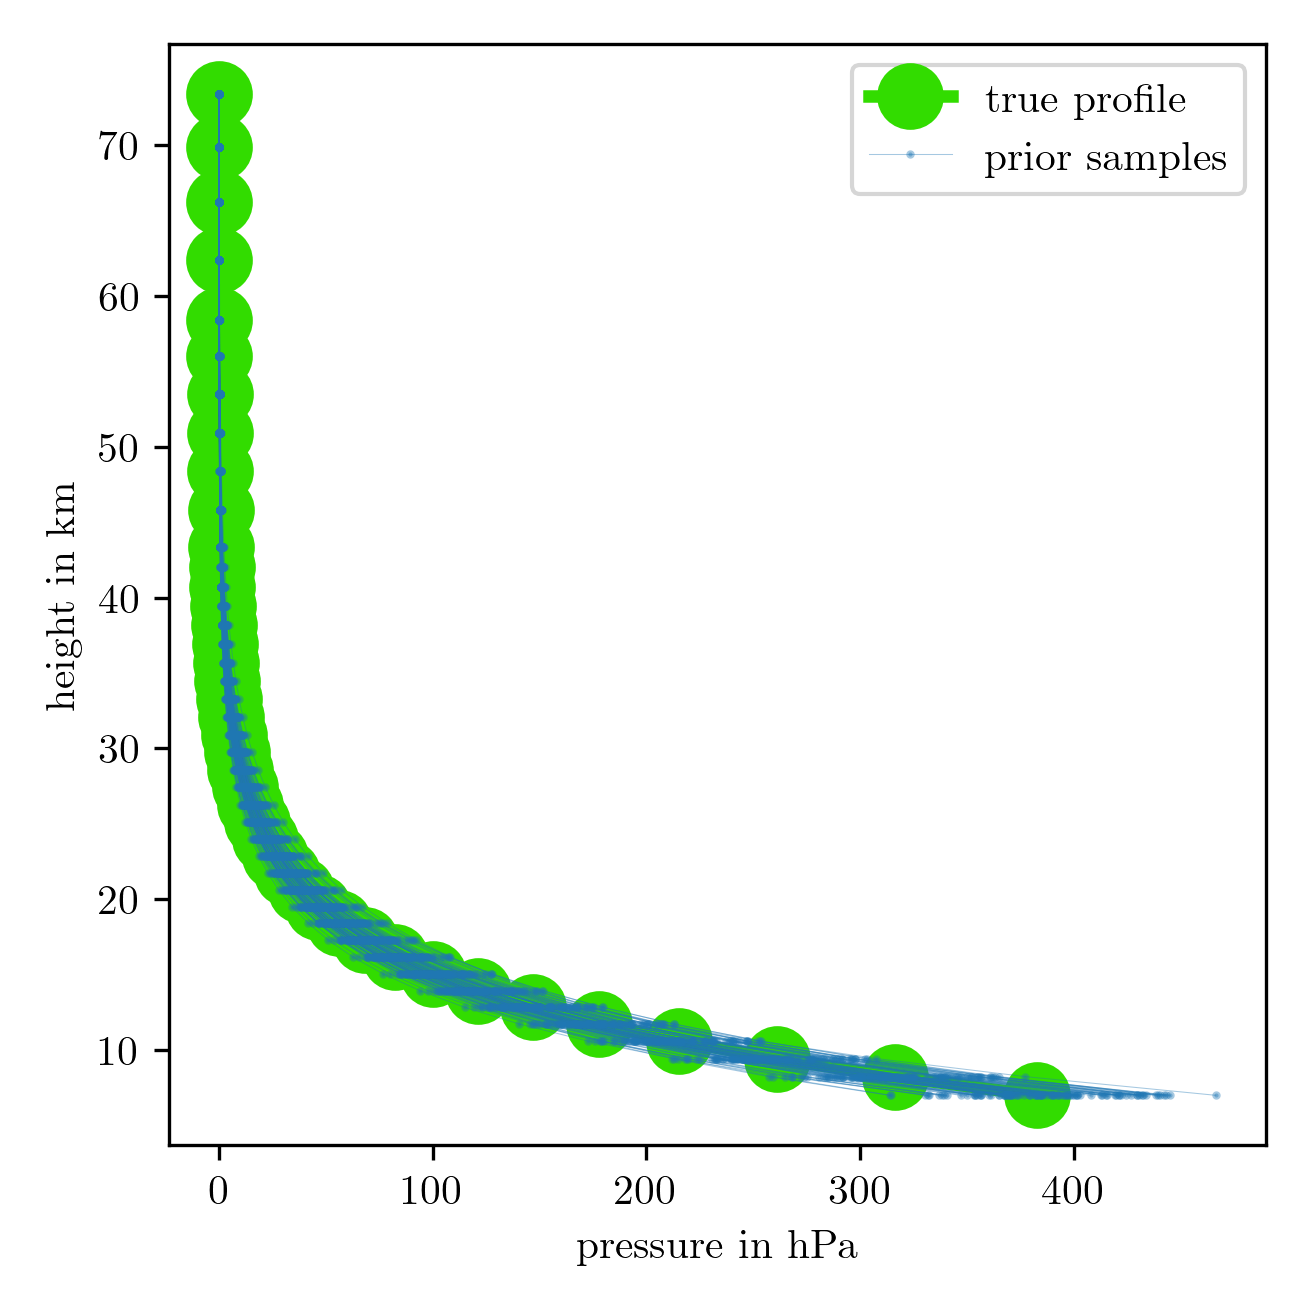
\includegraphics{PriorPressPostMeanSigm.png}
	\caption[Prior Samples of $\bm{p}$ according to the respective hyper-prior distribution.]{Prior samples from the hyper-prior distribution of $b$ and $p_0$ as defined in Tab.~\ref{tab:priors}, where we calculate $\bm{p}$ according to the function in Eq.~\ref{eq:pressFunc}.}
	\label{fig:PriorPress}
\end{figure}
\begin{figure}[ht!]
	\centering
	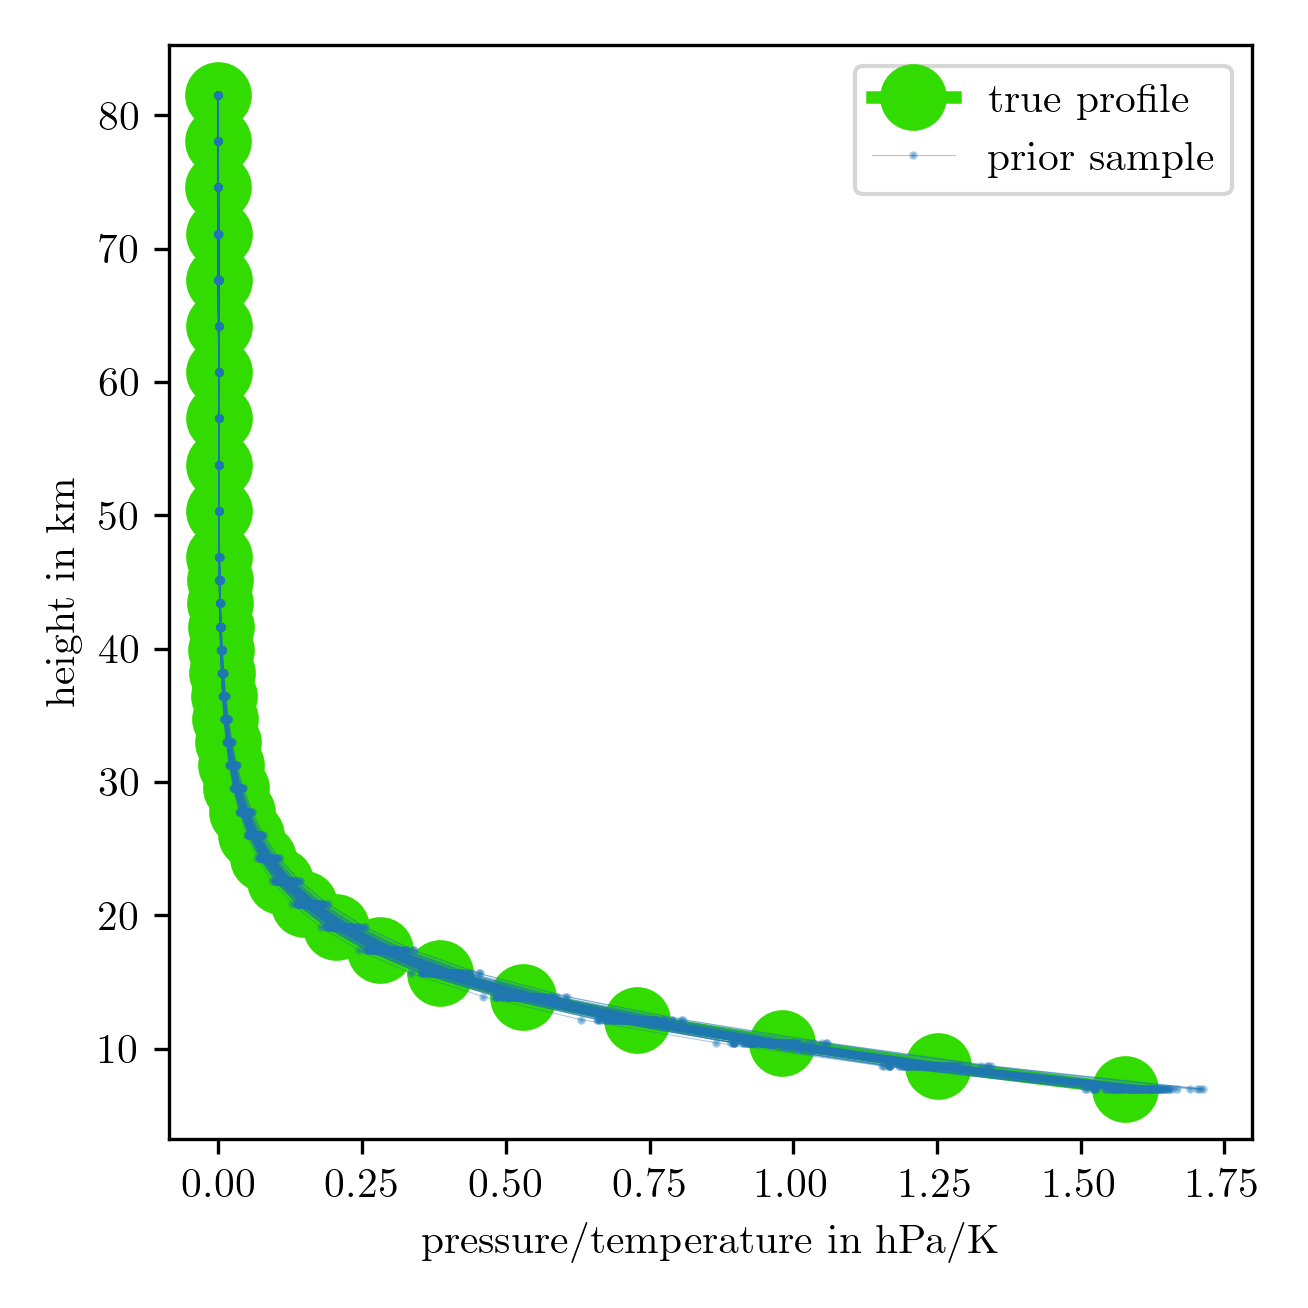
\includegraphics{PriorTempOverPostMeanSigm.png}
	\caption[Prior Samples of $\bm{p}/\bm{T}$ according to the respective hyper-prior distribution.]{Prior samples from the hyper-prior distribution of $\bm{h}_T$, $\bm{a}$ and $T_0$ for temperature as in Eq.~\ref{eq:tempFunc} and $b$ and $p_0$ for pressure as in Eq.~\ref{eq:pressFunc}. We plot $\bm{p}/\bm{T}$. The hyper-priors are defined in Tab.~\ref{tab:priors}.}
	\label{fig:PriorPressOverTemp}
\end{figure}
We observe that the pressure $\bm{p}$ in between $h_{L,0} \approx 7$km and $h_{L,n} \approx 83$km can be described with an exponential function
\begin{align}
	p(h) =
	\exp \left( -b \, h \right)   \,  p_0 \quad , \text{$h_{L,0}  \leq h \leq h_{L,n}$}
	\label{eq:pressFunc}
\end{align}
depending on two hyper-parameters $p_0,b$ (see Fig.~\ref{fig:PriorPress}).
Similarly, the temperature as described in Eq.~\ref{eq:tempFunc} can be parametrised with 14 hyper-parameters\linebreak $\bm{h}_T = \{ h_{T,1}, h_{T,2},h_{T,3},h_{T,4},h_{T,5},h_{T,6} \}$, $\bm{a} = \{a_0, a_1, a_2,a_3,a_4,a_5,a_6 \} $ and $T_0$ (see Fig.~\ref{fig:PriorTemp} and Eq.~\ref{eq:tempFunc}).

The hyper-prior distributions for $p_0,b, T_0,\bm{h}_T ,\bm{a} $ are defined to be Gaussians, and to complete the model we have to choose sensible hyper-prior variances and means.
The variances of $\pi(\bm{h}_T)$ are tuned so that the temperature profile maintains its structure and $ h_{T, i} < h_{T, i+1}$, for $i = 1,\dots, 5$ (see Fig.~\ref{fig:HeightPriors}).
The means of $\pi(\bm{h}_T)$ and $\pi(\bm{a})$ are set to ground truth values see Tab.~\ref{tab:tempGrad} and the variances of $\pi(\bm{a})$ allow a wide range of prior temperature profiles.
Similarly, the variance and mean of $\pi(T_0)$ are chosen to mimic a daily temperature variability of roughly $30$K around the mean sea level temperature $288$K~\cite{atmosphere1976us}.
These hyper-prior distributions are rather informative, because we find that the data and the model (see Fig.~\ref{fig:PriorPressOverTemp}) are uninformative about the temperature profile.
The variance of $\pi(b)$ is set to a rather large value.
The variability of $\pi(p_0)$ is $\approx 80$hPa and close to what we can observe when looking at weather data.
Means for $\pi(b ,p_0)$ are provided by fitting the exponential in Eq.~\ref{eq:pressFunc} to ground truth pressure values via the Python function \texttt{scipy.optimize.curve\_fit}.
The in Sec.~\ref{subsec:PriorModelO3} defined Gamma distributions $\pi(\delta,\gamma)$ are not changing, so that scale and rate are $\{  \alpha_\gamma, \beta_\gamma\}  = \{ \alpha_\delta ,\beta_\delta\} = (1,10^{-35})$.
See Tab.~\ref{tab:priors} for a summary of the hyper-prior distributions.

Prior samples against their ground truth profiles of the pressure $\bm{p}$ are plotted in Fig.~\ref{fig:PriorPress}, the temperature $\bm{T}$ in Fig.~\ref{fig:PriorTemp}, the ratio $\bm{p}/\bm{T}$ in Fig.~\ref{fig:PriorPressOverTemp} and additionally prior samples of $1/\bm{T}$ are plotted in Fig.~\ref{fig:OverTempPrior}.
In Fig.~\ref{fig:PriorPressOverTemp} we already observe that $\bm{p}/\bm{T}$ inherits the structure of the pressure function and hence the model is uninformative about the temperature.
\clearpage
%Note that we fit one exponential function to ground truth pressure values between $h_{L,0} \approx 7$km and $h_{L,n} \approx 82$, so that the pressure value $p_0$ may be different to true sea-level pressure values at $h = 0$km due to that approximation.
\section{Posterior Distribution}
Here, the marginal posterior and the full conditional posterior distribution for the described Bayesian model are formulated.
We either use the t-walk algorithm~\cite{christen2010general} to draw samples from the marginal posterior $\pi(p_0,b,T_0,\bm{h_T},\bm{a} ,\lambda, \gamma| \bm{y})$ with $\lambda = \delta / \gamma$ or we utilise a TT approximation on a predefined grid to generate samples via the SIRT method with an MH correction step.
In doing so, the reader is guided through the process of obtaining an efficient TT approximation and some key aspects are pointed out. 
Lastly, the RTO method is utilised to draw ozone samples from the full conditional posterior $\pi(\bm{x}|p_0,b,T_0,\bm{h_T},\bm{a} ,\lambda, \gamma, \bm{y})$.
Recall that the linear forward model matrix is $\bm{A}_{\bm{\theta}}$ is depending on the hyper-parameter defined as $\bm{\theta}  \coloneqq \{p_0,b,T_0,\bm{h_T},\bm{a}  \}$.
%Consequently, the marginal posterior is denoted as $\pi( \bm{\theta},\lambda,\gamma  | \bm{y}) $ and the full conditional posterior as $\pi(\bm{x}|\bm{\theta}, \lambda, \gamma, \bm{y})$.
\begin{table}[ht!]
	\centering
	\begin{tabular}{ |c||c|c|c|c|c|   }
		\hline
		& &\multicolumn{2}{|c|}{TT bounds}& t-walk&\\
		\hline
		model parameters& priors&\makecell{lower}& \makecell{upper\\
		}&$\tau_{\text{int}}$&Context\\
		\hhline{|=||=|=|=|=|=|}
		$\bm{x}$ &$\mathcal{N}(0,(\delta \bm{L})^{-1})$ & -&-&-& $\bm{x}$\\ \hline
		$\delta$ &$\mathcal{T}(1,10^{-35})$ & -&-&  -& $\bm{x}$\\ \hline
		$\gamma$ & $\mathcal{T}(1,10^{-35})$ &$8\times10^{14}$ &$1.2\times10^{16}$&  $ 507\pm 29$ &$\bm{y}$\\ \hline
		$\lambda  = \delta / \gamma$ &- & $1\times10^{-5}$&$2.5\times10^{-3}$& $979 \pm 75$ & -\\ \hline
		$b$ &  $\mathcal{N}(0.174,(0.01)^2)$& 0.129& 0.214 &$830\pm 60$&$\bm{p}$\\ \hline
		$h_{T,1}$ &  $\mathcal{N}(11,(1.5)^2)$&5.4 &16.3&$286\pm 13$ &$\bm{T}$\\ \hline
		$T_{0}$ &  $\mathcal{N}(288.15,(10)^2)$& 247 &326&$279 \pm 12$&$\bm{T}$\\ \hline
		$p_0$ &  $\mathcal{N}(1311,(20)^2)$&1237 &1387&$279\pm 12$&$\bm{p}$\\ \hline
		$h_{T,3}$ &  $\mathcal{N}(32.3,(2.5)^2)$&22.9&41.7&$254\pm 11$&$\bm{T}$\\ \hline
		$a_{1}$ &  $\mathcal{N}(0,(0.1)^2)$&-0.38 &0.38&$295 \pm 13$&$\bm{T}$\\ \hline
		$h_{T,2}$ &  $\mathcal{N}(20.1,(0.7)^2)$&17.2 &22.7&$296\pm 13$&$\bm{T}$\\ \hline
		$a_{0}$ &  $\mathcal{N}(-6.5,(0.01)^2)$&-6.54 &-6.47&$252 \pm 10$&$\bm{T}$\\ \hline
		$a_{2}$ &  $\mathcal{N}(1,(0.01)^2)$&0.97 &1.03&$267 \pm 11$&$\bm{T}$\\ \hline
		$a_{3}$ &  $\mathcal{N}(2.8,(0.1)^2)$&2.5 &3.1&$267\pm 11$&$\bm{T}$\\ \hline
		$h_{T,4}$ &  $\mathcal{N}(47.4,(0.5)^2)$&45.5 &49.3&$270 \pm 12$&$\bm{T}$\\ \hline
		$a_{4}$ &  $\mathcal{N}(0,(0.1)^2)$&-0.38 &0.38&$254 \pm 11$&$\bm{T}$\\ \hline
		$h_{T,5}$ &  $\mathcal{N}(51.4,(0.5)^2)$&49.5 &53.3&$280 \pm 12$&$\bm{T}$\\ \hline
		$a_{5}$ &  $\mathcal{N}(-2.8,(0.1)^2)$&-3.18 &-2.43&$278 \pm 12$&$\bm{T}$\\ \hline
		$h_{T,6}$ &  $\mathcal{N}(71.8,(3)^2)$&60.5 &83.1&$250\pm 10$&$\bm{T}$\\ \hline
		$a_{6}$ & $\mathcal{N}(-2,(0.01)^2)$ &-2.04 &-1.96&$272\pm 12$&$\bm{T}$\\
		\hline
	\end{tabular}
	\caption[Summary of relevant parameter characteristics, bounds and sampling statistics.]{Summary of relevant parameter and hyper-parameters bounds and statistics, ordered as in the TT format according to their correlation structure. We denote $\mathcal{N}(\mu= \text{mean},\sigma^2= \text{variance})$ as the Gaussian and $\mathcal{T}(\alpha = \text{scale}, \beta = \text{rate})$ as the Gamma distribution. The IACT $\tau_{\text{int}}$ from marginal posterior samples via the t-walk is twice the value provided by~\cite{UwerrM, drikHesse}.}
	\label{tab:priors}
\end{table}
\clearpage

\subsection{Marginal Posterior -- Pressure and Temperature}
The marginal posterior is given as
\begin{align}
	\pi( \bm{\theta},\lambda,\gamma  | \bm{y}) \propto &  \lambda^{n/2} \gamma^{m/2}   \exp{ \Bigl\{ - \frac{1}{2} g ( \bm{\theta},\lambda) - \frac{\gamma}{2} f (\bm{\theta},\lambda) \Bigr\}} \pi(\bm{\theta},\lambda,\gamma ) \, ,
	\label{eq:MargPostFull}
\end{align}
with $\lambda= \delta / \gamma$,
\begin{subequations}
	\label{eq:fandgTrue}
	\begin{align}
		&f ( \bm{\theta},\lambda) = \bm{y}^T \bm{y} - \big(\bm{A}_{\bm{\theta}}^T \bm{y}\big)^T \big(\bm{A}_{\bm{\theta}}^T  \bm{A}_{\bm{\theta}} + \lambda \bm{L}\big)^{-1} \big(\bm{A}_{\bm{\theta}}^T \bm{y}\big)  \label{eq:fFullAppl} \, ,  \\
		&\text{and } g(\bm{\theta},\lambda) = \log \det \big(\bm{A}_{\bm{\theta}}^T  \bm{A}_{\bm{\theta}} + \lambda \bm{L}\big) \label{eq:gFullAppl} \, .
	\end{align}
\end{subequations}
For each evaluation of $\pi( \bm{\theta},\lambda,\gamma  | \bm{y})$, $\bm{A}_{\bm{\theta}}$ is composed as in Chapter~\ref{ch:formodel}, and $f$ and $g$ are calculated directly using the Cholesky decomposition via the Python functions \texttt{np.linalg.cholesky} and \texttt{scy.linalg.cho\_solve}.

\subsubsection{Sampling from the marginal posterior}
Since the hierarchical model has $18$ hyper-parameters, we utilise the t-walk algorithm by Christen and Fox~\cite{christen2010general} to sample from the marginal posterior $\pi(\bm{\theta} , \lambda, \gamma| \bm{y})$, because it is quick-to-implement and easy-to-use.
The t-walk chooses between four different types of steps on the target distribution.
It is employed as a black-box algorithm in default settings, requiring the specification of the number of samples, burn-in period, support region, and the target distribution. 
Convergence to the target distribution is guaranteed by the construction of this algorithm~\cite{christen2010general}.

Running the t-walk algorithm with the objective to generate $1000$ independent samples from the marginal posterior provides a ground truth to which we compare the TT approximation.
The maximum IACT provided by twice the value of \cite{wolff2004monte, drikHesse} (see Tab.~\ref{tab:priors} and Fig.~\ref{fig:TWalkIATC1} to Fig.~\ref{fig:TWalkIATC18}) can be bounded by $1100$.
Then the t-walk takes $N = 1000 \times 1100$ steps plus a burn-in period of $N_{\text{burn-in}} = 100 \times 1100 $ for $1000$ independent samples.
We initialise the Python implementation of the t-walk~\cite{christentwalkaccess} around the hyper-prior mean values and the mode of $\pi(\lambda ,\gamma|\bm{y})$ (see Sec.~\ref{subsec:MWG} and e.g., Fig.~\ref{fig:ScatterPlotTT}).
For a total number of $N + N_{\text{burn-in}} = 1210000$ steps within iteratively defined hyper-parameter support bounds (see TT bounds in Tab.~\ref{tab:priors}) a time of $\approx 10$ mins is taken.
The resulting histograms are plotted in Fig.~\ref{fig:PostHistTT0} to Fig.~\ref{fig:PostHistTT4} and the output trace of the marginal posterior in Fig.~\ref{fig:TraceTwalk}.
\begin{figure}[ht!]
	\centering
	\includegraphics{TraceTwalk.png}
	\caption[T-walk trace]{Output trace of samples from the marginal posterior distribution $\pi(\bm{\theta},\lambda,\gamma|\bm{y})$ via the t-walk.}
	\label{fig:TraceTwalk}
\end{figure}
\clearpage

\subsubsection{TT approximation of marginal posterior}
The aim now is to approximate the square root of the marginal posterior
\begin{align}
	\begin{split}
		\sqrt{\pi( \bm{\theta},\lambda,\gamma  | \bm{y})} \propto  \exp\Bigl\{ 0.5\log{\pi( \bm{\theta},\lambda,\gamma  | \bm{y}) } + c \Bigr\}  
	\end{split} 
	\label{eq:MargPostFullTT}
\end{align}
with a ``normalisation constant'' $c=-200$ to stay within computer precision.
In doing so, we run the~\texttt{tt.cross.rectcross.rect\_cross.cross} Python function from the \texttt{ttpy} Python package \cite{Oseledets2018ttpy} on a grid (see TT bounds in Tab.~\ref{tab:priors}) according to the results of the t-walk. 
We observe marginal posterior values around $10^{27}$ so we set $\xi = 1 / \uplambda (\mathcal{X})$ with $\uplambda(x) = 1$.
For Cartesian basis the mass matrix becomes $\bm{M}_k = \text{diag}(\uplambda_k(\mathcal{X}_k))$.
To draw samples from the TT approximation the SIRT-MH scheme is used as introduced in Sec.~\ref{subsec:SamplTT}.

\cleardoublepage
\paragraph{Correlation structure}
First, we order the hyper-parameters according to their correlation structure to improve the efficiency of the TT approximation. 
Specifically, the hyper-parameter space $\mathcal{X}_{\gamma} \times \mathcal{X}_{\lambda} \times \mathcal{X}_{b} \times \cdots$ is arranged in such a way that highly correlated hyper-parameter pairs are adjacent and directly linked through their shared TT rank.
For samples via the SIRT-MH, twice the value of~\cite{wolff2004monte, drikHesse} provides an average IACT of $\approx 1.2 \pm 0.2$.
Hence 1000 independent samples from the marginal posterior require 2000 samples via the SIRT-MH scheme.
In Fig.~\ref{fig:CorrPlot} those 1000 samples and the Pearson correlation coefficients between hyper-parameter pairs are plotted.
A coefficient close to $1$ or $-1$ indicates strong correlation, while values near zero suggest weak or no correlation.
We observe that the hyper-parameters $\lambda$ and $b$, and $\lambda$ and $\gamma$ are highly correlated.
Additionally, $h_{T,1}$ describing the temperature at low altitudes (strong signal) is mildly correlated to $b$.
This is because $h_{T,1}$ influences ``the smoothness'' of $\bm{p}/\bm{T}$, which is hard to see in Fig.~\ref{fig:PriorPressOverTemp}.
Interestingly, $p_0$ appears largely uncorrelated with other hyper-parameters, while $b$ is the key parameter linking pressure to ozone and temperature.
Hyper-parameters describing the temperature at higher altitudes are very much uncorrelated and the IACTs of the t-walk in Tab.~\ref{tab:priors} agree with those results.
Alternatively, one could decorrelate the hyper-parameter space using a coordinate system rotation e.g.,~via Cholesky whitening~\cite{KessyWhitening2018}.
\clearpage
\begin{figure}[h!]% will be the left-side figure
	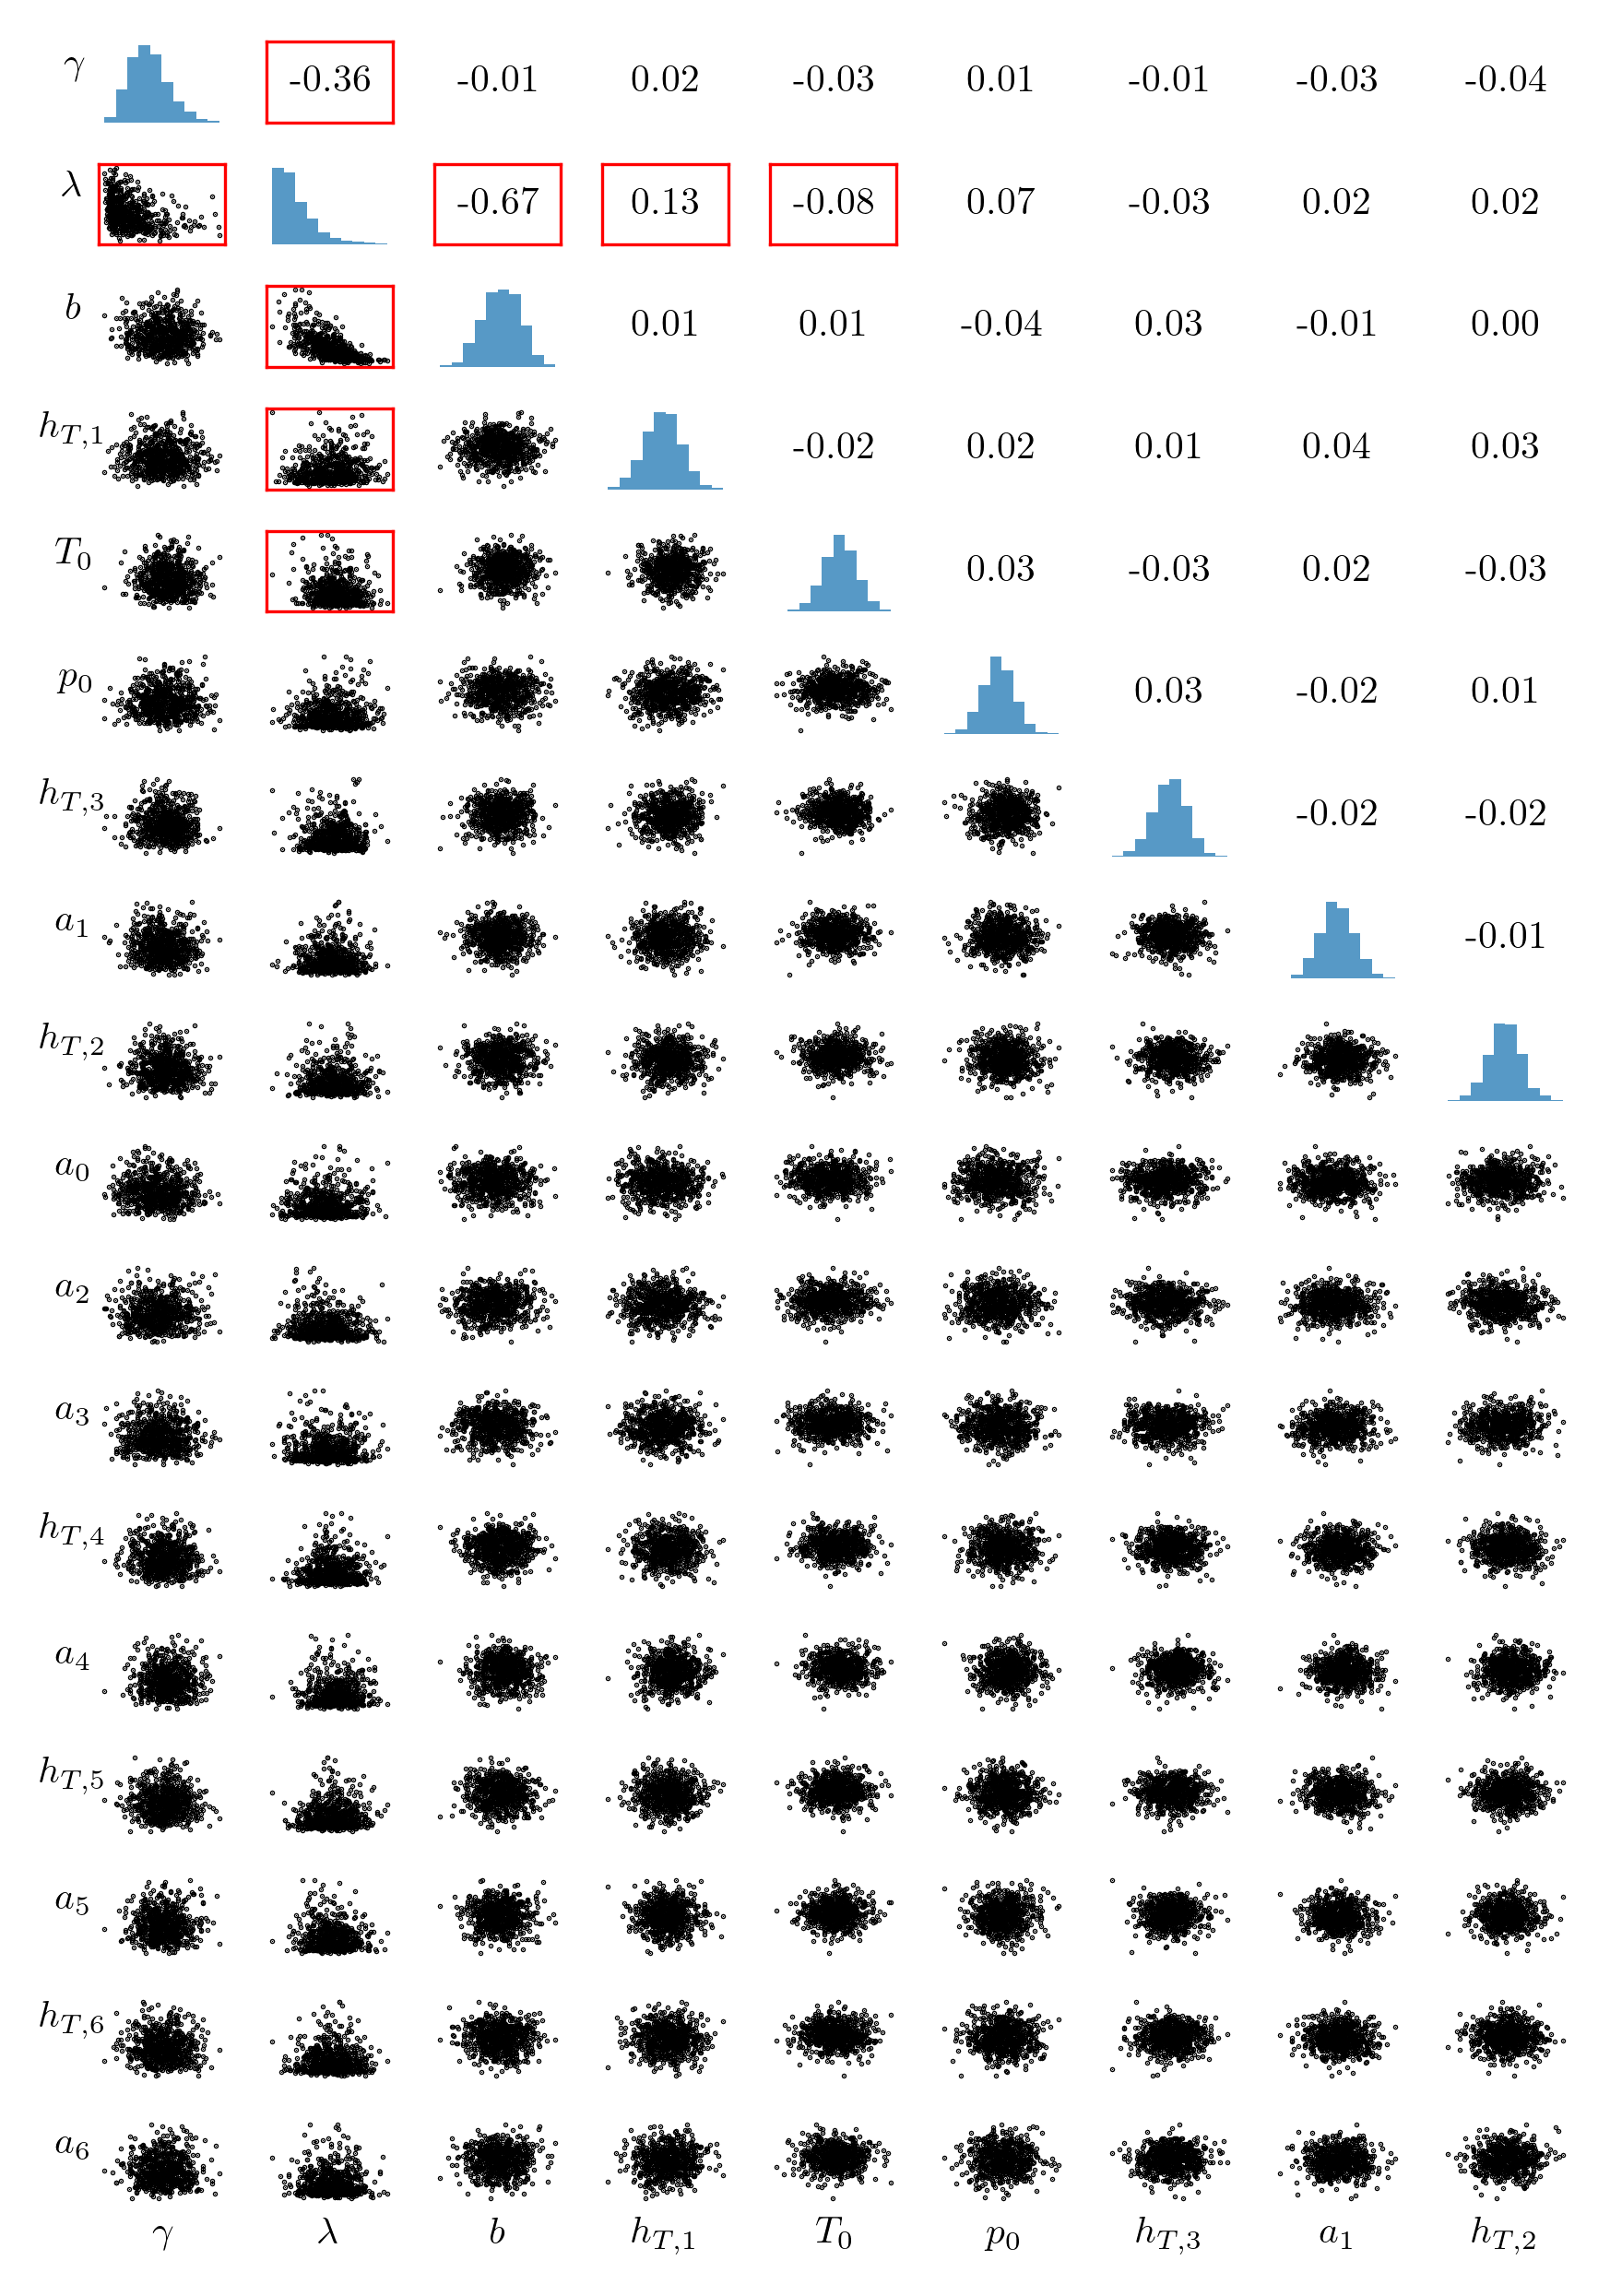
\includegraphics[]{CorrPlot.png}
	\caption[Correlation plot of samples from TT approximation]{Plot of 1000 independent samples from TT approximation of $\sqrt{\pi( \bm{\theta},\lambda,\gamma  | \bm{y})}$ via SIRT-MH scheme. We plot the Pearson correlation coefficient ranging from $-1$ to $1$ for each hyper-parameter pair.}
	\label{fig:CorrPlot}
\end{figure}
\begin{figure}% will be the right-side figure
	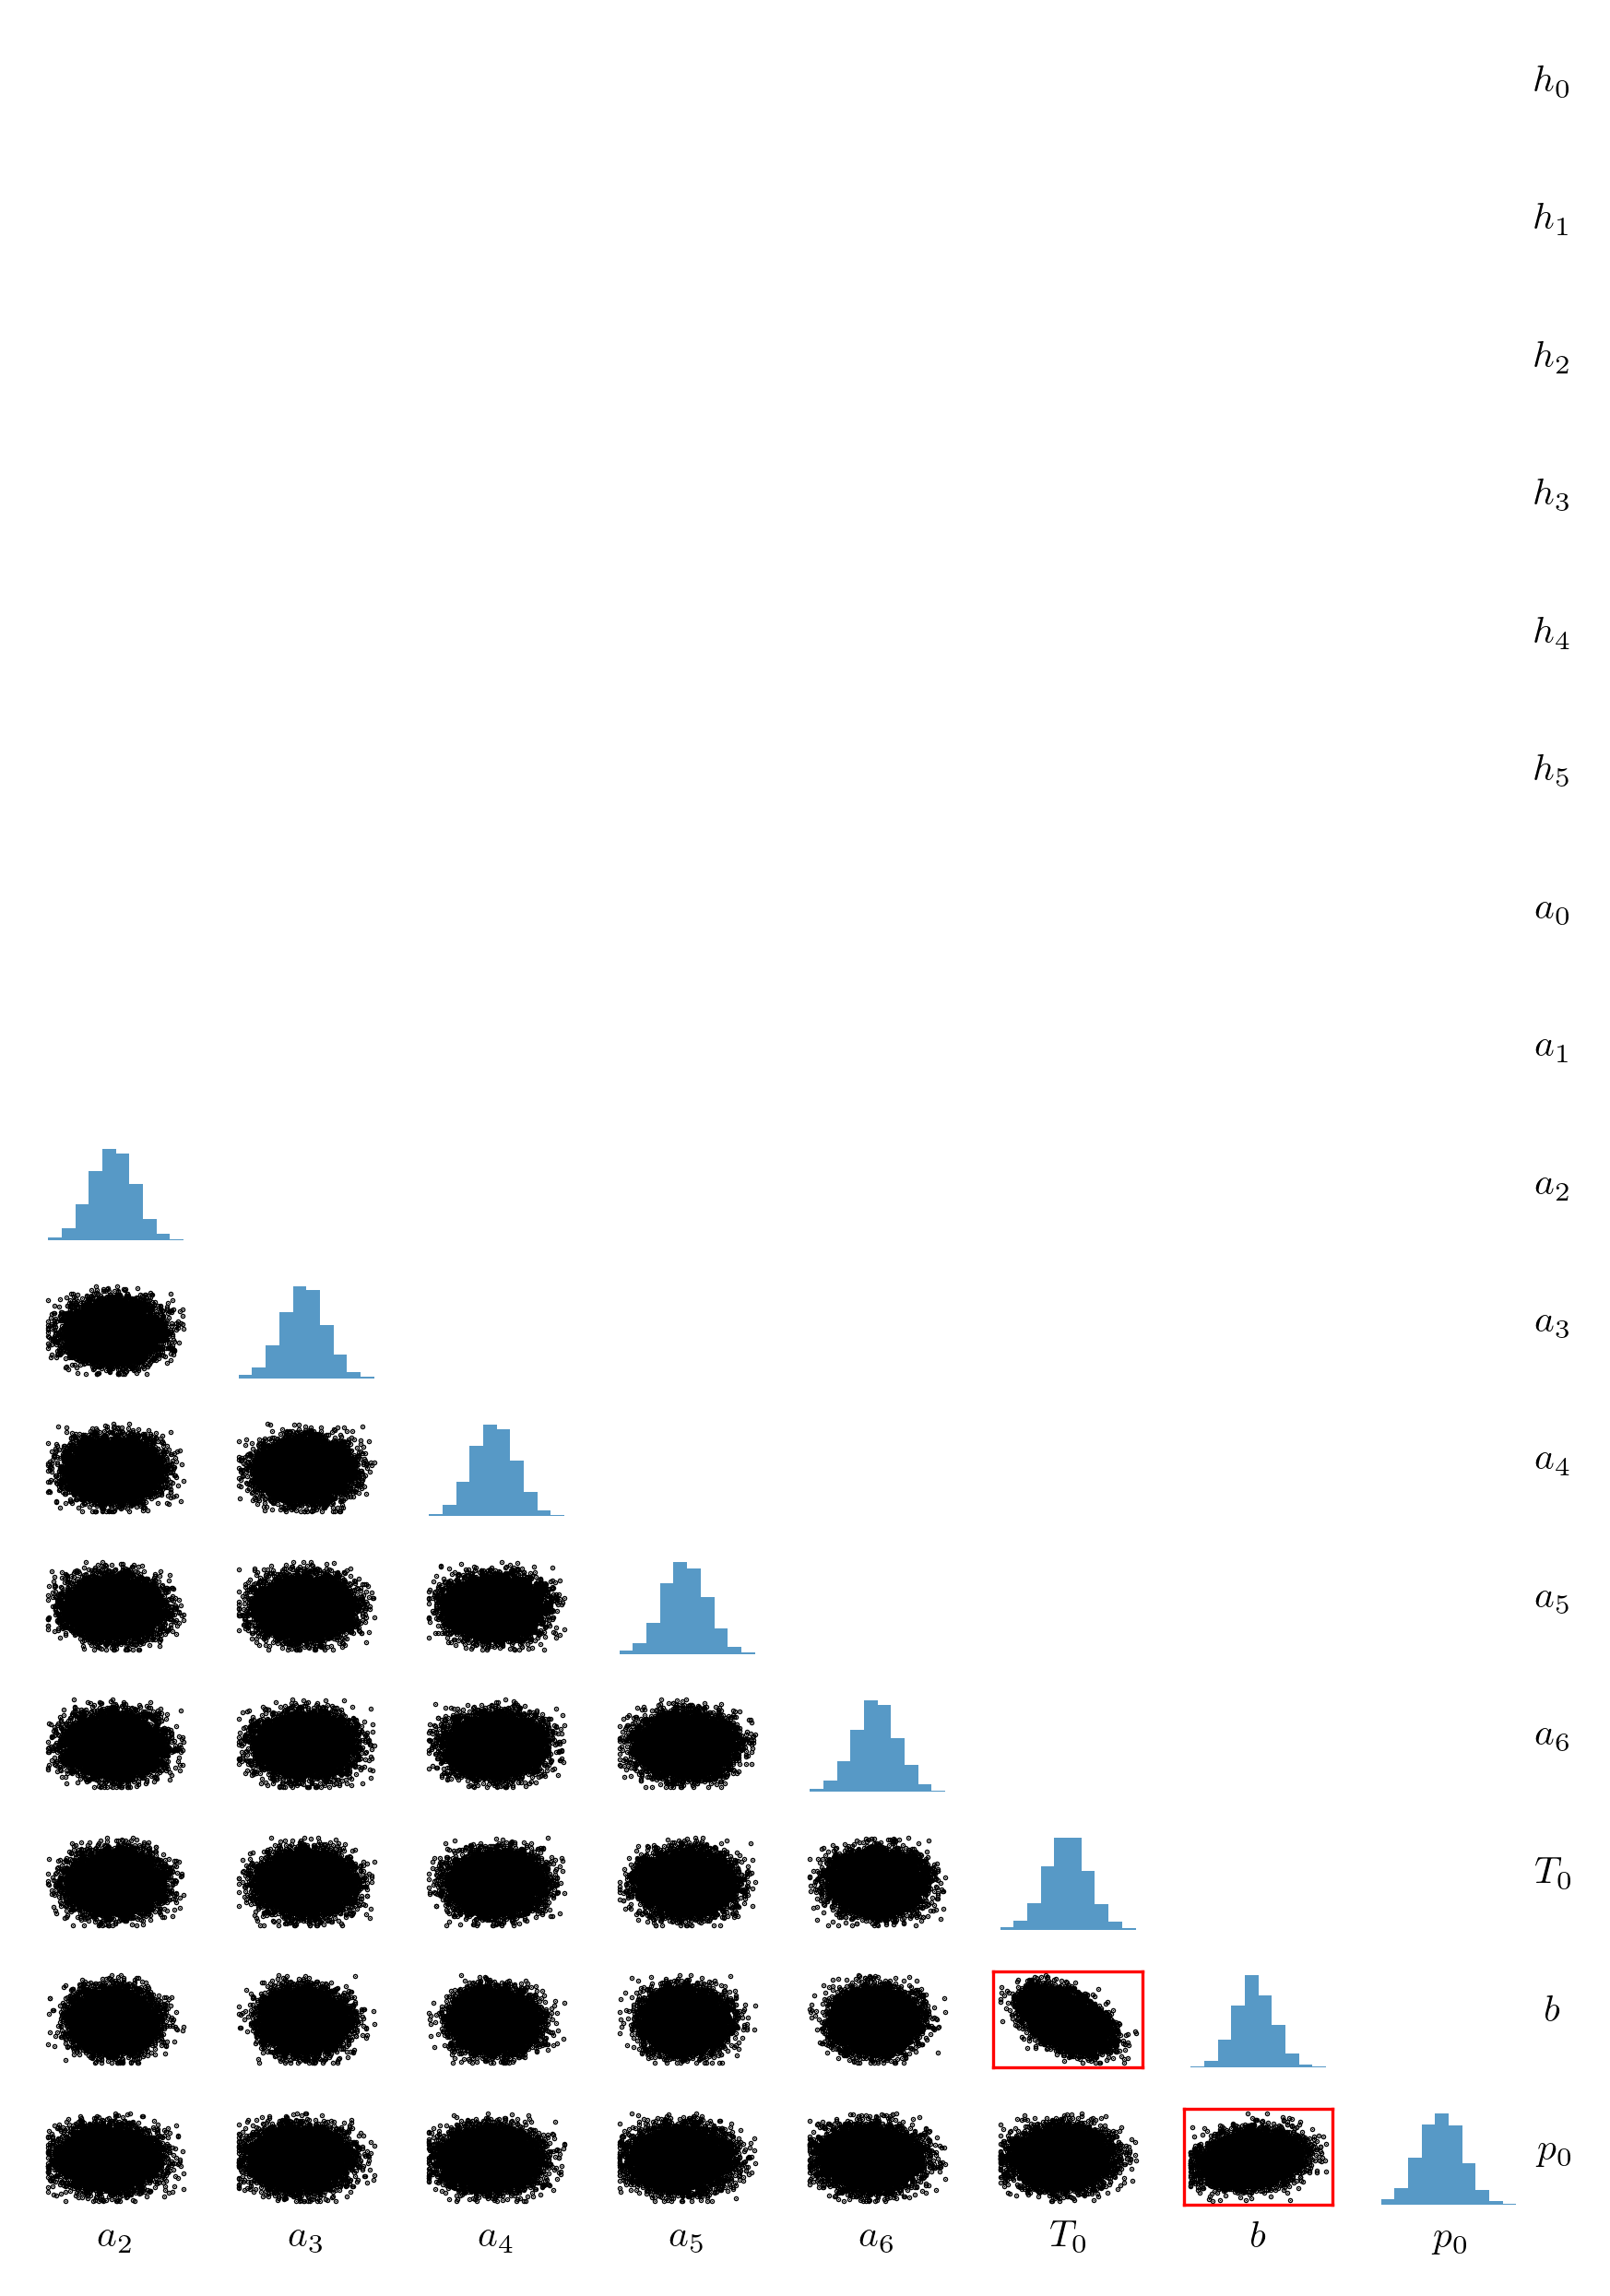
\includegraphics[]{2ndCorrPlot.png}
	\caption*{Correlation plot of samples from TT-approximation of $\sqrt{\pi(\bm{\theta},\lambda,\gamma | \bm{y})}$ via SIRT-MH scheme.}
\end{figure}



\paragraph{Find optimal rank and grid size}
The aim is to approximate $\pi( \bm{\theta},\lambda,\gamma  | \bm{y})$ with a number of marginal posterior evaluations as small as possible but without losing too much accuracy.
In doing so, the number of grid points is set to $n = 150$ and different error measures for ranks $\{2,3,4,5,6,7,8,9,10,11,12,13,14,15, 20, 25, 30, 35, 50\}$ are calculated.
For a fixed low rank, the number of grid points $\{10, 15, 20, 25, 30, 35, 40, 45, 50, 55, 60, 65, 70, 80, 90, 100\}$ is decreased until sufficient accuracy.

For stable and comparable results, we do five sweeps within \linebreak the~\texttt{tt.cross.rectcross.rect\_cross.cross} Python function initialised at a random TT.
The ranks between TT cores are constant.
Then $N = 1000$ independent samples  $ \{( \tilde{ \bm{\theta}},  \tilde{\lambda},  \tilde{\gamma })^{(1)} ,\dots, (\tilde{ \bm{\theta}},  \tilde{\lambda},  \tilde{\gamma })^{(N)}   \} \sim \tilde{\pi}( \bm{\theta},\lambda,\gamma  | \bm{y})$ from the TT approximation $\tilde{\pi}( \bm{\theta},\lambda,\gamma  | \bm{y})$ via the SIRT-MH scheme are drawn.
The sample mean is denoted as $\bm{\mu}_{\text{SIRT-MH}}\in \mathbb{R}^{18}$.
Further, the marginal functions from the TT approximation are used to calculate the hyper-parameter mean $\bm{\mu}_{\text{TT}}\in \mathbb{R}^{18}$ by weighted expectations via quadrature.

For a ground truth $N = 1000$ samples $ \{( \bm{\theta},\lambda,\gamma )^{(1)} ,\dots,( \bm{\theta},\lambda,\gamma )^{(N)}   \} \sim \pi( \bm{\theta},\lambda,\gamma  | \bm{y})$
are obtained from the t-walk and the sample mean is denoted as $ \bm{\mu}_{\text{t-walk}}  \in \mathbb{R}^{18}$.
The true marginal posterior is denoted as $ \pi( \bm{\theta},\lambda,\gamma  | \bm{y})$.

Plotted in Fig.~\ref{fig:FindRankGrid}, for each TT approximation, the following error measures are calculated:
\begin{itemize}
	\item[{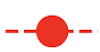
\includegraphics[height=0.65\baselineskip]{SIRTMH.png}}] The average \textbf{relative expectation error (SIRT-MH)}
	\begin{align*} 
		\frac{\lVert\bm{\mu}_{\text{SIRT-MH}} - \bm{\mu}_{\text{t-walk}} \rVert_{L^2}}{  \lVert \bm{\mu}_{\text{t-walk}} \rVert_{L^2} } \, .
	\end{align*}
	\item[{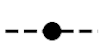
\includegraphics[height=0.65\baselineskip]{QUAD.png}}] The average \textbf{relative expectation error (quadrature)}
	\begin{align*} 
		\frac{\lVert\bm{\mu}_{\text{TT}} - \bm{\mu}_{\text{t-walk}} \rVert_{L^2} }{ \lVert \bm{\mu}_{\text{t-walk}} \rVert_{L^2} } \, .
	\end{align*}
	\item[{
\includegraphics[height=0.65\baselineskip]{RMS.png}}] The \textbf{relative RMS error} 
	\begin{align*} 
		\frac{\lVert \tilde{\pi}(\tilde{ \bm{\theta}},  \tilde{\lambda},  \tilde{\gamma})  - \pi(\tilde{ \bm{\theta}},  \tilde{\lambda},  \tilde{\gamma}) \rVert_{L^2} }{ \lVert \pi(\tilde{ \bm{\theta}},  \tilde{\lambda},  \tilde{\gamma})  \rVert_{L^2} } \, .
	\end{align*}
	\item[{
\includegraphics[height=0.65\baselineskip]{W1.png}}] The \textbf{1-Wasserstein distance}
	\begin{align*} 
		W_1(\pi,\tilde{\pi}) = 	\underset{\nu \in \Pi(\pi,\tilde{\pi}) }{\text{min}} \sum^N_{i,j =1}  \nu_{ij} \lVert \text{vec}\big(( \bm{\theta},\lambda,\gamma ) ^{(i)} \big)-  \text{vec}\big( (\tilde{ \bm{\theta}},  \tilde{\lambda},  \tilde{\gamma})^{(j)}\big) \rVert_{L^2} \, .
	\end{align*}
\end{itemize} 
The 1-Wasserstein distance as in Eq.~\ref{eq:applWasser} is calculated between 1000 independent SIRT-MH samples from the TT approximation $\tilde{\pi}( \bm{\theta},\lambda,\gamma  | \bm{y})$ weighted by their approximated values and 1000 independent t-walk samples from the true marginal posterior weighted by $\pi( \bm{\theta},\lambda,\gamma  | \bm{y})$.
Here $\text{vec}( \bm{\theta},\lambda,\gamma )$ denotes the vector of hyper-parameters $\big( \bm{\theta}^T,\lambda^T,\gamma^T \big)^T \in \mathbb{R}^{18}$ and $\nu_{ij} \coloneqq  \tilde{\pi}\big( (\tilde{ \bm{\theta}},  \tilde{\lambda},  \tilde{\gamma})^{(j)}   | \bm{y}\big)  \pi\big( (\bm{\theta},\lambda,\gamma )^{(i)}  | \bm{y}\big) $.
As in~\cite{feydy2020OT} we normalise over the samples so that $\sum \pi\big( (\bm{\theta},\lambda,\gamma )^{(i)}  | \bm{y}\big)  = 1$ and $\sum \tilde{\pi}\big( (\tilde{ \bm{\theta}},  \tilde{\lambda},  \tilde{\gamma})^{(j)}   | \bm{y}\big) = 1$.
The Python function \texttt{SamplesLoss("sinkhorn", p=$1$, blur=$0.05$, scaling=0.8)} with default settings from the Python package \texttt{geomloss}~\cite{Wassersteinaccess} is used to obtain $W_1$.
This function provides the unbiased Sinkhorn divergence which converges towards the Wasserstein distance and can be understood as the generalised Quicksort algorithm~\cite{feydy2020OT}.
Here p$ = 1$ defines the distance measure $\lVert \cdot \rVert_{L^2}$.
The blur parameter is an entropic penalty, and the scaling parameter specifies the trade-off between speed (scaling $< 0.4$) and accuracy (scaling $>0.9$)~\cite{Wassersteinaccess}.
The relative RMS Error between approximated marginal posterior values and true marginal posterior values is calculated at sample points provided by the SIRT-MH scheme.
See~\cite{dolgov2020approximation}, for using the mean rejection rate of the MH correction steps as an indicator for the average absolute error.



\begin{figure}[ht!]
	\centering
	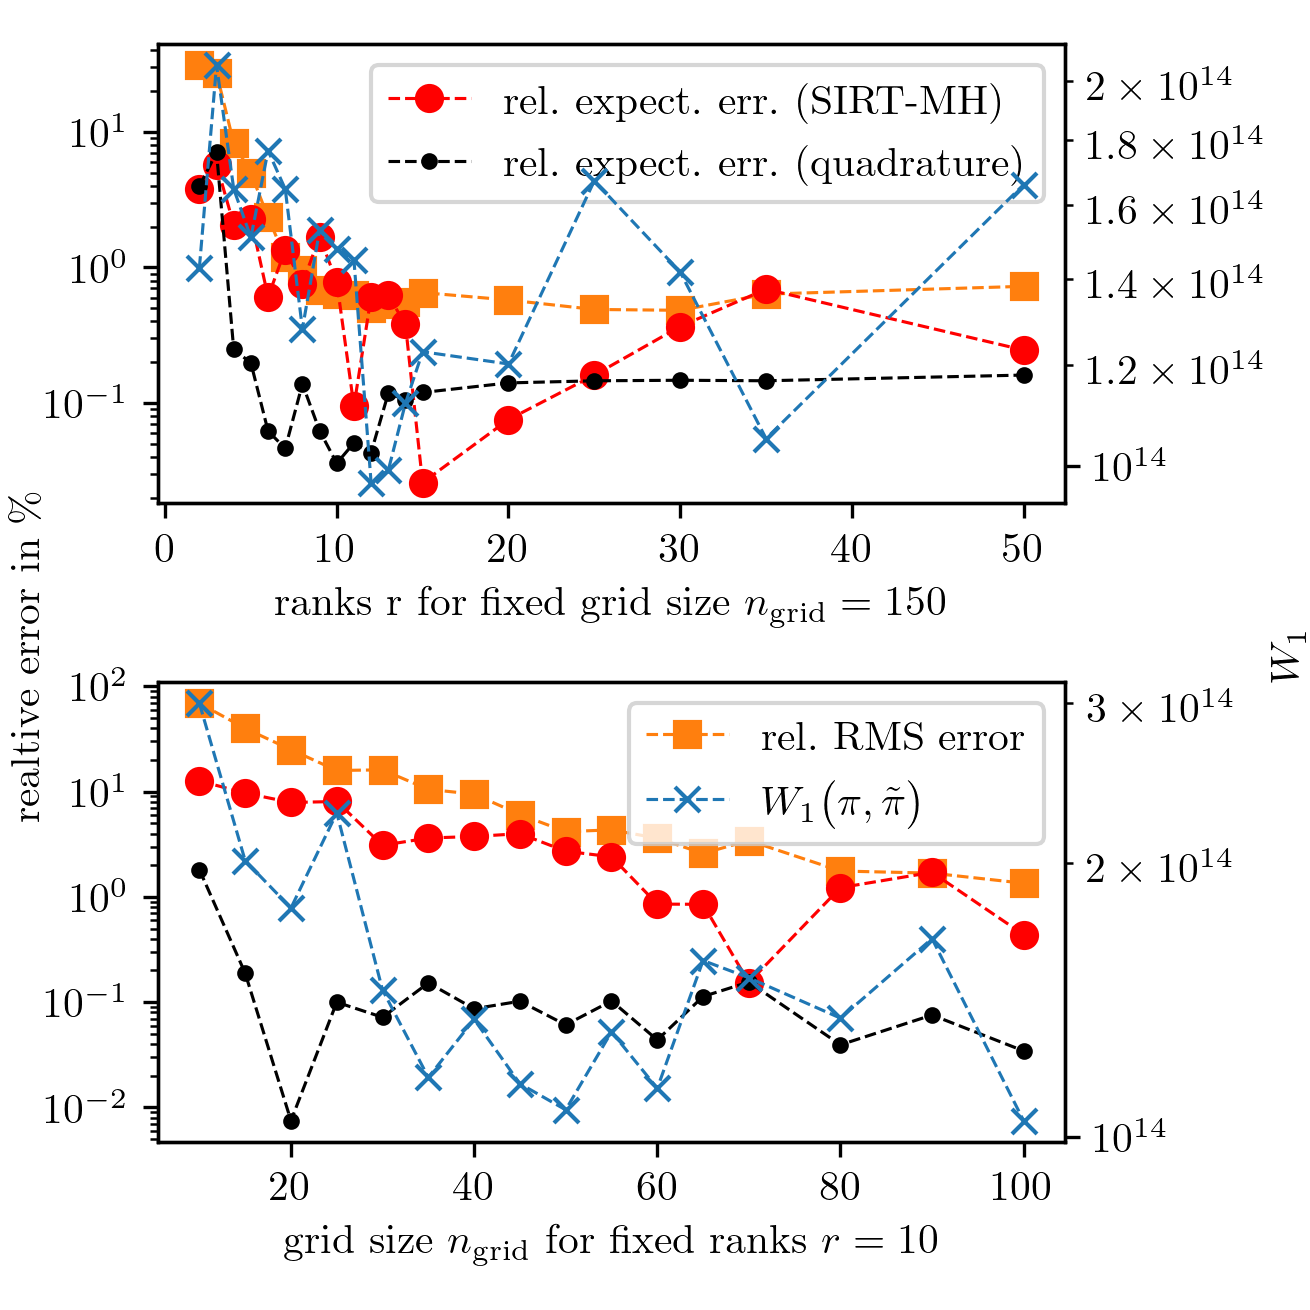
\includegraphics[]{findGridRank.png}
	\caption[Optimal rank and number of grid points for TT approximation.]{Given the TT approximations of $\sqrt{\pi( \bm{\theta},\lambda,\gamma  | \bm{y}) }$ four different error measures are calculated (see list in text).
		For a fixed grid size, the ranks are increased until sufficient accuracy of the TT approximation.
		Then with a fixed rank the grid size is increased and the error measures are plotted to choose a large enough number of grid points.}
	\label{fig:FindRankGrid}
\end{figure}
 
In Fig.~\ref{fig:FindRankGrid}, we observe that a rank $r = 10$ is sufficient because the error measures are relatively stable for $r\geq10$.
For a grid size $n \geq 30$ the relative differences between $\bm{\mu}_{\text{TT}}$ and $\bm{\mu}_{\text{t-walk}}$ (red circles in Fig.~\ref{fig:FindRankGrid}) and the RMS errors at the 1000 independent SIRT-MH samples (orange squares in Fig.~\ref{fig:FindRankGrid}) are around $ 10\%$ and considered good enough.
For an increasing number of grid points the interpolation of function values between grid points is more accurate, and the relative RMS and sample based expectation error decrease.
This is because the chosen linear interpolation (see Eq.~\ref{eq:LinPol}) is a rather rudimentary choice.
The quadrature-based relative expectation error (black dots in Fig.~\ref{fig:FindRankGrid}) is almost constant for ranks $ \gtrsim 7$ and grid sizes $ > 20$.
This indicates that the accuracy of the TT approximation is relatively stable and most of the error is due to interpolation between grid points.
Since the hyper-parameters have different length scales, we are only interested in the trend of the sample-based 1-Wasserstein distance (blue crosses in Fig.~\ref{fig:FindRankGrid}).
The 1-Wasserstein distance is quite fluctuant but decreases with increasing ranks and stays within a similar range for grid sizes $n \geq 30$.


\begin{figure}[ht!]
	\centering
	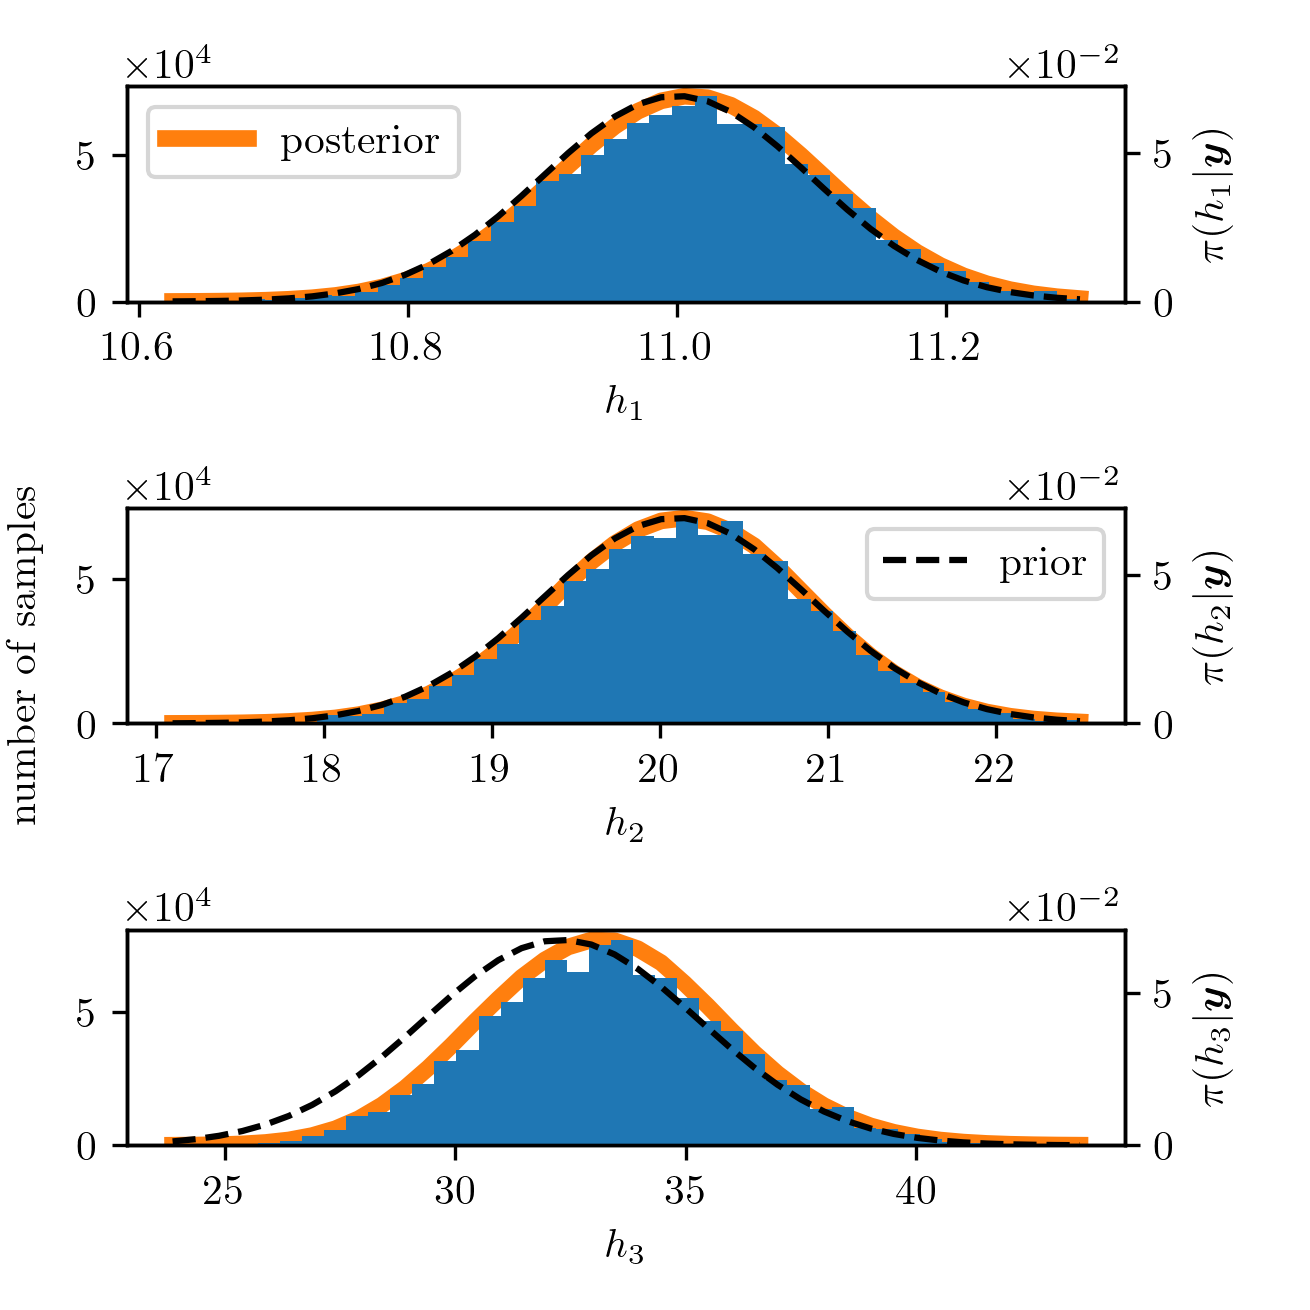
\includegraphics{PHdPTPost0.png}
	\caption[Histograms and TT approximation of posterior distribution as well as hyper-prior distribution.]{Plot of the TT approximation of the marginal posterior in orange and the samples from the t-walk as a histogram. The prior distribution is plotted as a dotted line.}
	\label{fig:PostHistTT0}
\end{figure}
\begin{figure}[ht!]
	\centering
	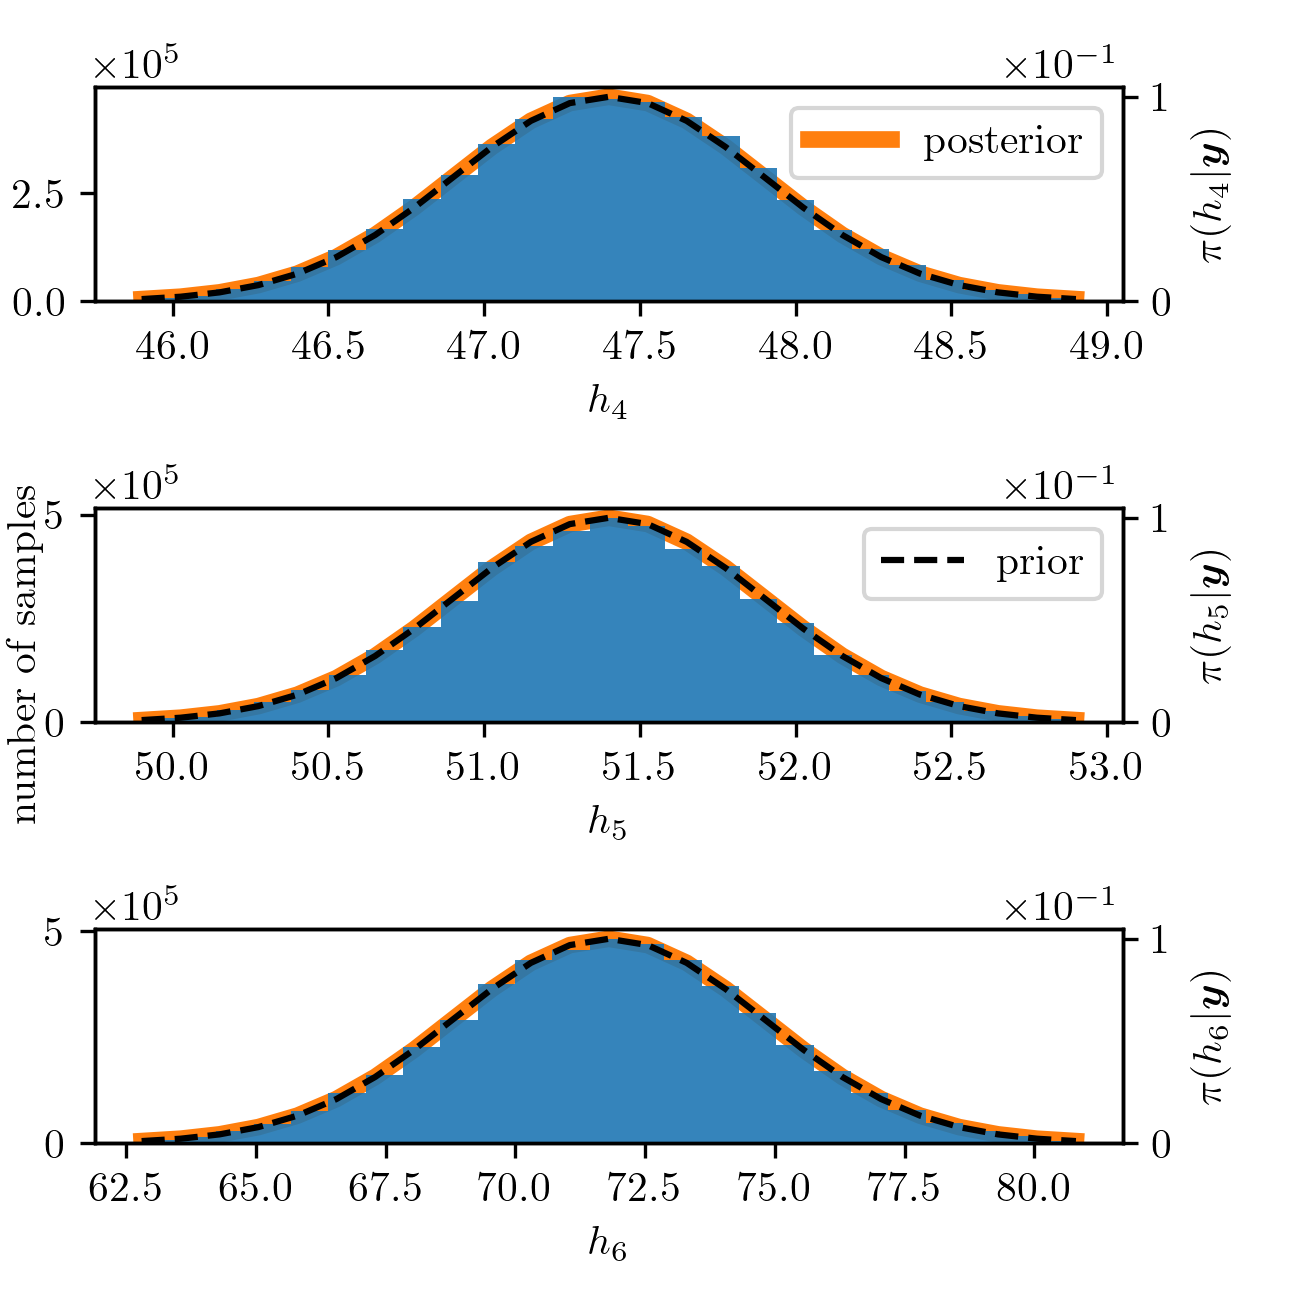
\includegraphics{PHdPTPost1.png}
	\caption[Histograms and TT approximation of posterior distribution as well as hyper-prior distribution.]{Plot of the TT approximation of the marginal posterior in orange and the samples from the t-walk as a histogram. The prior distribution is plotted as a dotted line.}
	\label{fig:PostHistTT1}
\end{figure}
\begin{figure}[ht!]
	\centering
	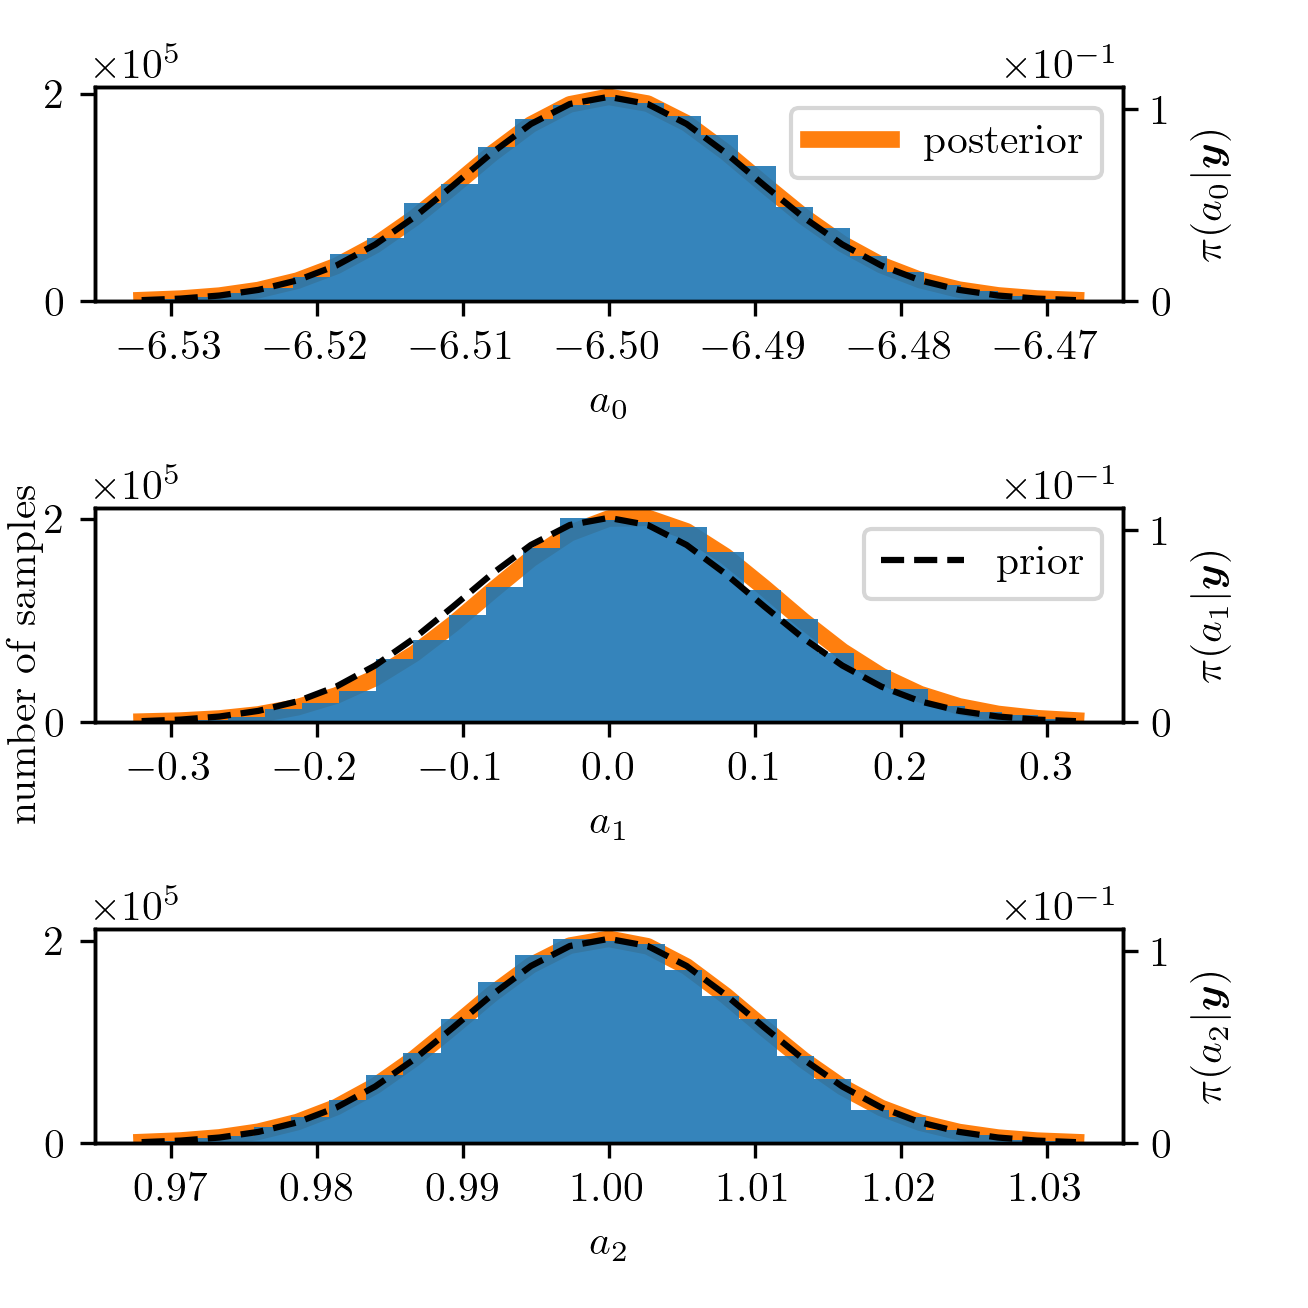
\includegraphics{PHdPTPost2.png}
	\caption[Histograms and TT approximation of posterior distribution as well as hyper-prior distribution.]{Plot of the TT approximation of the marginal posterior in orange and the samples from the t-walk as a histogram. The prior distribution is plotted as a dotted line.}
	\label{fig:PostHistTT2}
\end{figure}
\begin{figure}[ht!]
	\centering
	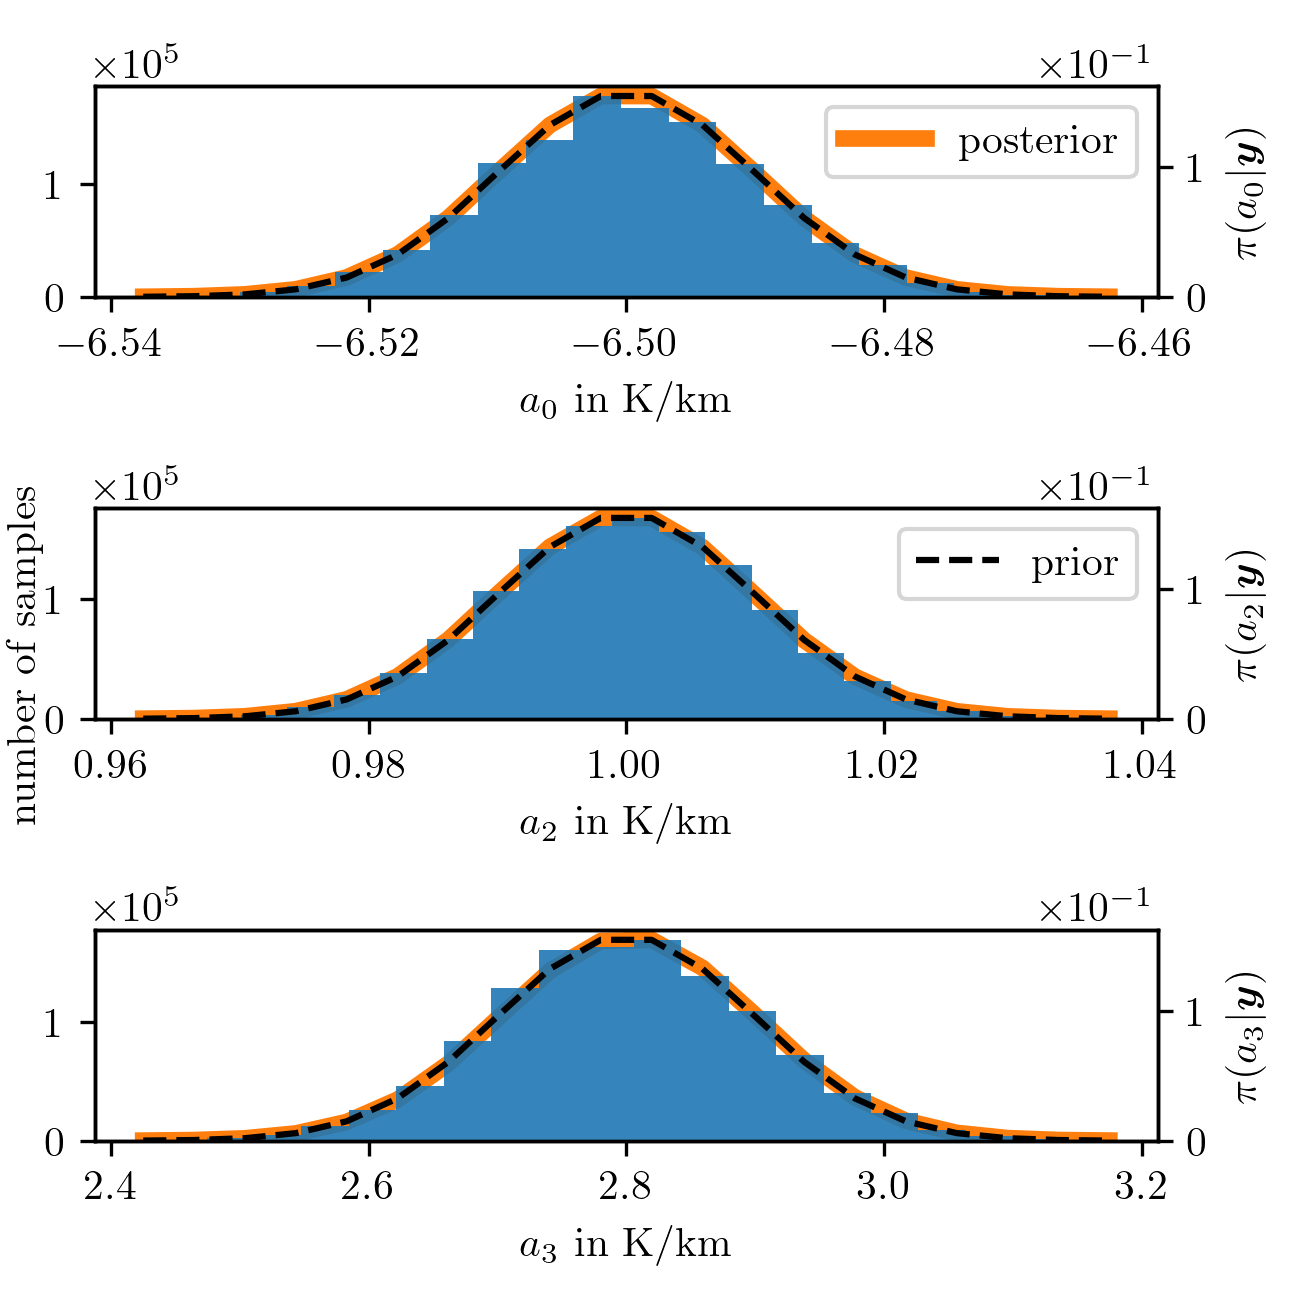
\includegraphics{PHdPTPost3.png}
	\caption[Histograms and TT approximation of posterior distribution as well as hyper-prior distribution.]{Plot of the TT approximation of the marginal posterior in orange and the samples from the t-walk as a histogram. The prior distribution is plotted as a dotted line.}
	\label{fig:PostHistTT3}
\end{figure}
\begin{figure}[ht!]
	\centering
	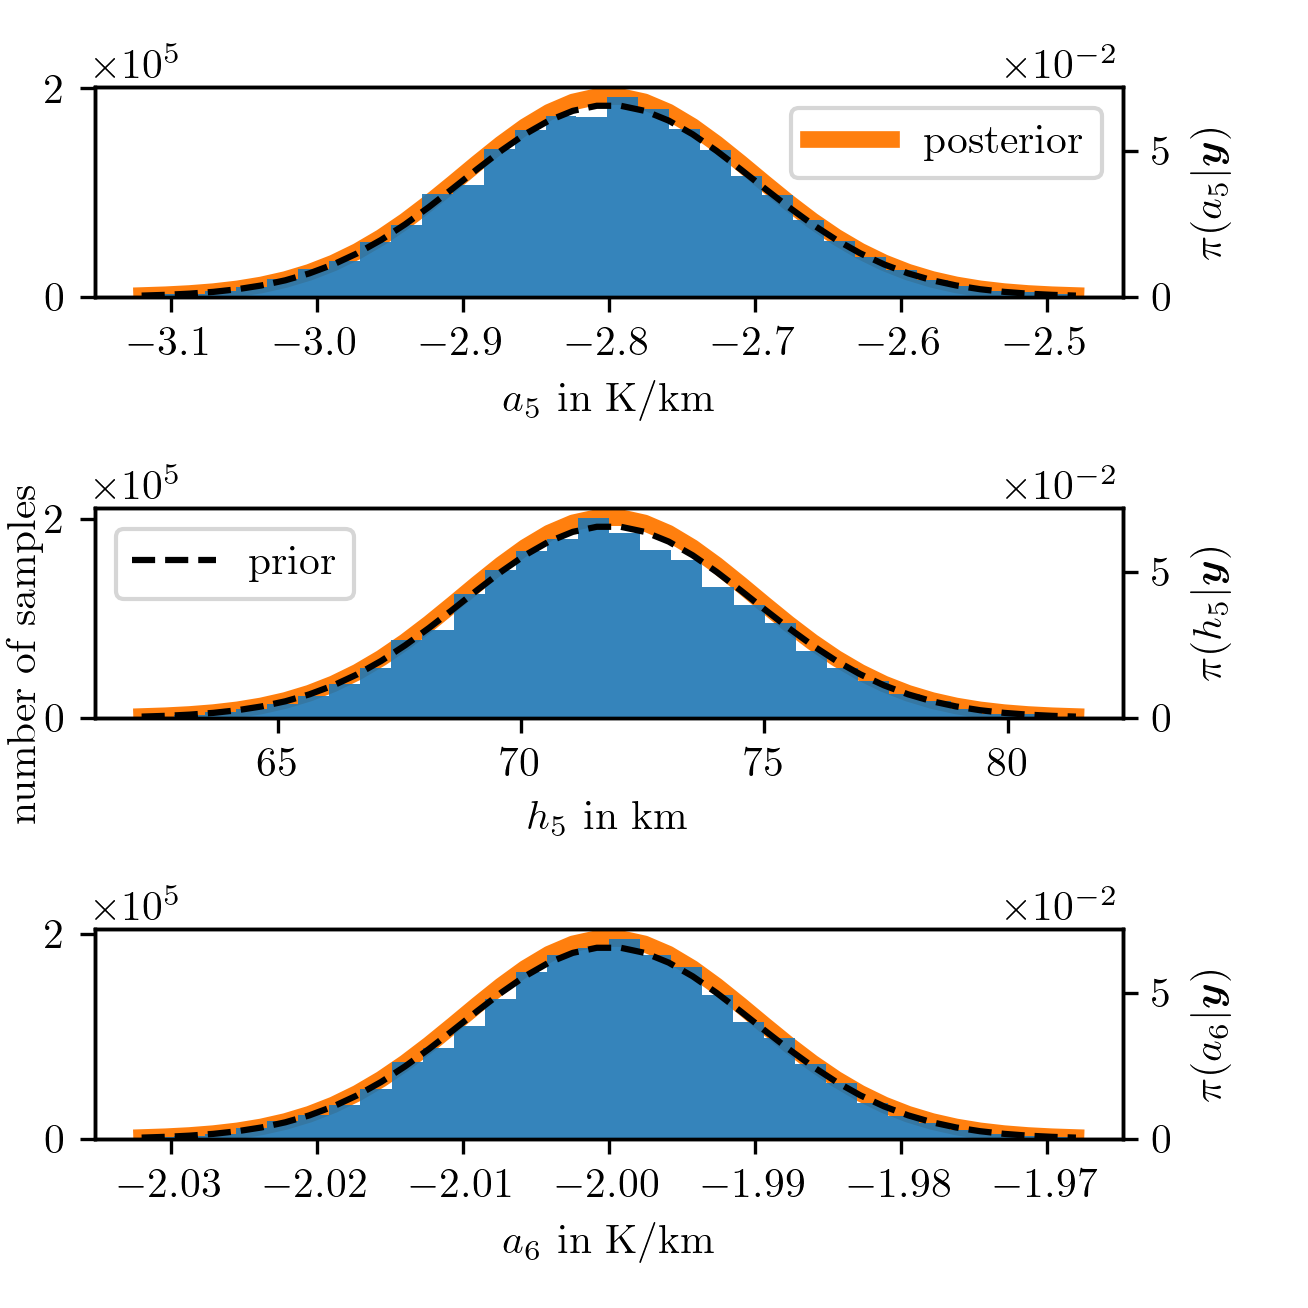
\includegraphics{PHdPTPost4.png}
	\caption[Histograms and TT approximation of posterior distribution as well as hyper-prior distribution.]{Plot of the TT approximation of the marginal posterior in orange and the samples from the t-walk as a histogram. The prior distribution is plotted as a dotted line.}
	\label{fig:PostHistTT4}
\end{figure}
\begin{figure}[ht!]
	\centering
	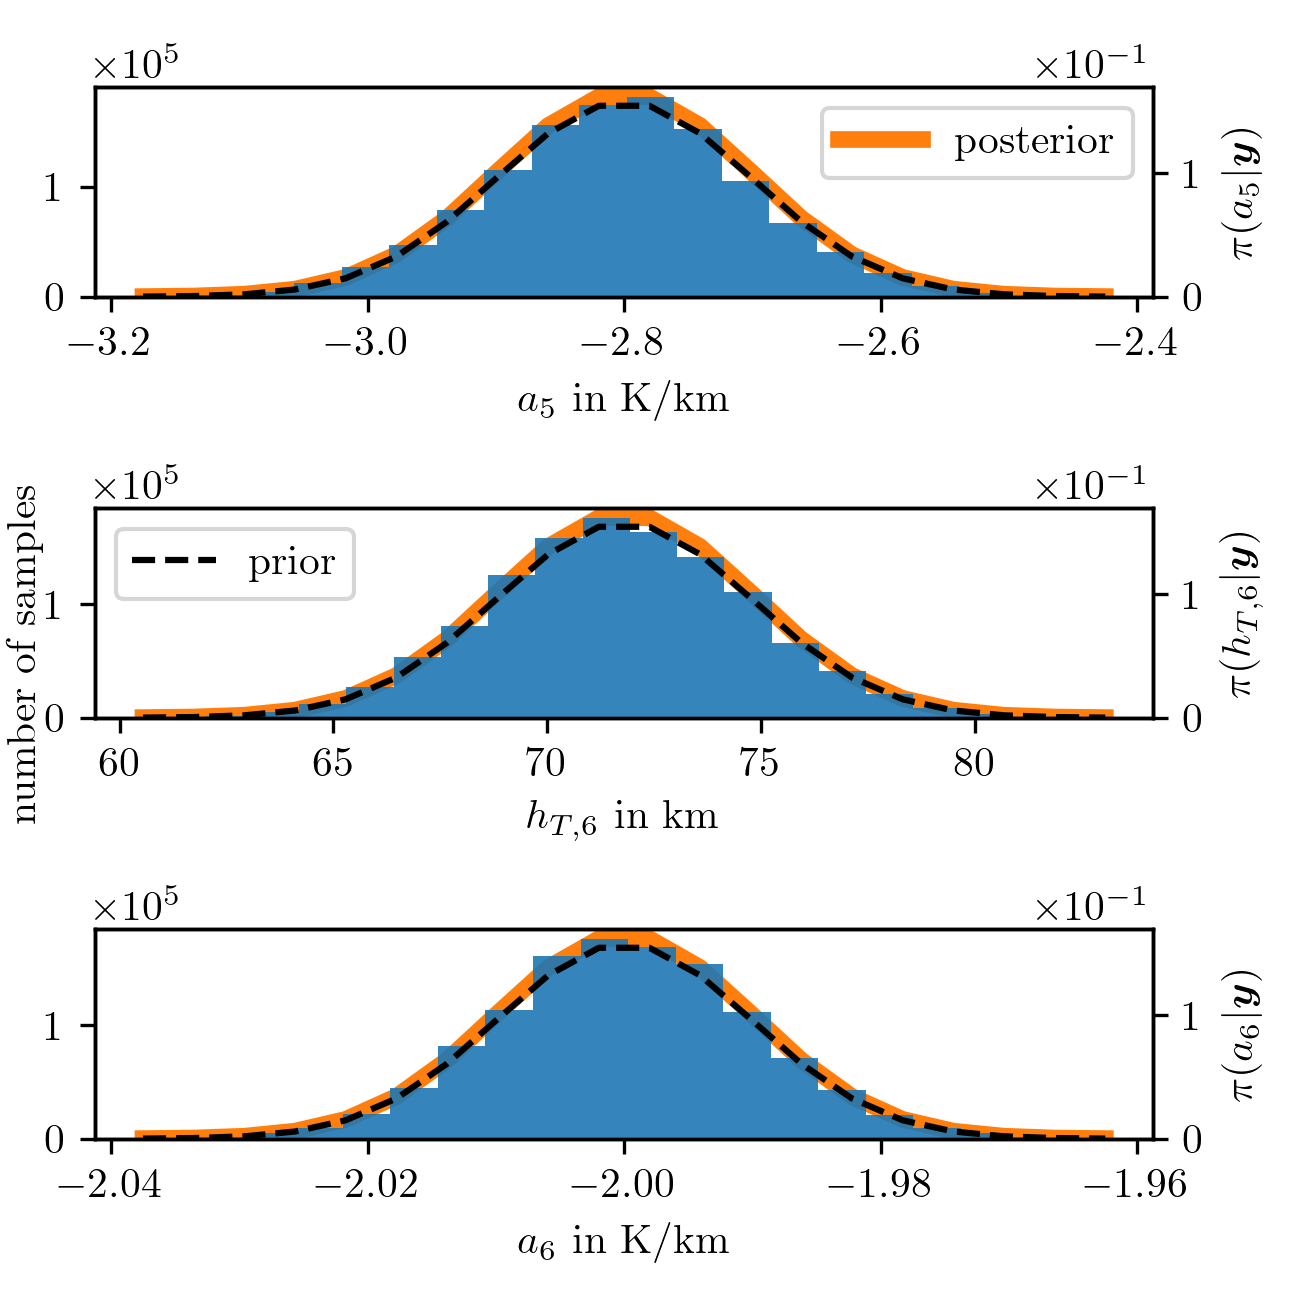
\includegraphics{PHdPTPost5.png}
	\caption[Histograms and TT approximation of posterior distribution as well as hyper-prior distribution.]{Plot of the TT approximation of the marginal posterior in orange and the samples from the t-walk as a histogram. The prior distribution is plotted as a dotted line.}
	\label{fig:PostHistTT5}
\end{figure}

Based on these results the grid size is set to $n = 30$.
Next, we define ranks $r =[ 1,  10,  10, 10, 10, 10, 5, 3, 3, 3, 3, 3, 3 , 3, 3, 3, 3, 3, 1]$ between TT cores, with a maximum rank of $10$.
This harvests the correlation structure of $\pi(\bm{\theta},\lambda,\gamma  | \bm{y})$ and decreases the number of marginal posterior evaluations even further.
One sweep in the\linebreak \texttt{tt.cross.rectcross.rect\_cross.cross} initialised at a previously calculated approximation reduces the computation time to $\approx 10$s and the number of marginal posterior evaluations to 34080.
For the samples drawn via the SIRT-MH scheme, the average IACT (provided by twice the value of~\cite{wolff2004monte, drikHesse}) is $\approx 1.2 \pm 0.2$.
This means that once the TT approximation is available, two function evaluations per independent sample are needed.
To draw 1000 independent samples, including generating a TT approximation, takes $\approx30$s.

We report a relative RMS error of $\approx 12 \%$ evaluated over those 1000 independent samples.
The relative RMS error over 1000 randomly chosen grid points is $\approx 1\%$, so the linear interpolation causes most of the approximation error.

The marginals for each hyper-parameter are plotted in Fig.~\ref{fig:PostHistTT0} to Fig.~\ref{fig:PostHistTT5}.
We observe that, besides $\lambda$ and $\gamma$, only the marginal posterior of the $b$ hyper-parameter is seriously affected by the data and has significantly changed compared to the hyper-prior distribution.
\clearpage

\subsubsection{Posterior pressure and temperature}
Posterior pressure and temperature profiles are directly obtained by hyper-parameter samples from the marginal posterior $\pi(\bm{\theta},\lambda,\gamma  | \bm{y})$ and according to their respective function (see Eq.~\ref{eq:tempFunc} and Eq.~\ref{eq:pressFunc}).
In Fig.~\ref{fig:PressPost} and Fig.~\ref{fig:TempPost}, 50 posterior profiles and the posterior sample mean from 1000
posterior samples are plotted.
The posterior temperature profiles look (as expected) similar to the prior temperature profiles.
The posterior pressure profiles have slightly larger values compared to the ground truth.
This is because the hyper-parameter $b$ is smaller than its ground truth value (see Fig.~\ref{fig:PostHistTT0}), resulting in the posterior pressure profiles that do not exponentially decrease as fast as the ground truth pressure profile.

\begin{figure}[ht!]
	\centering
	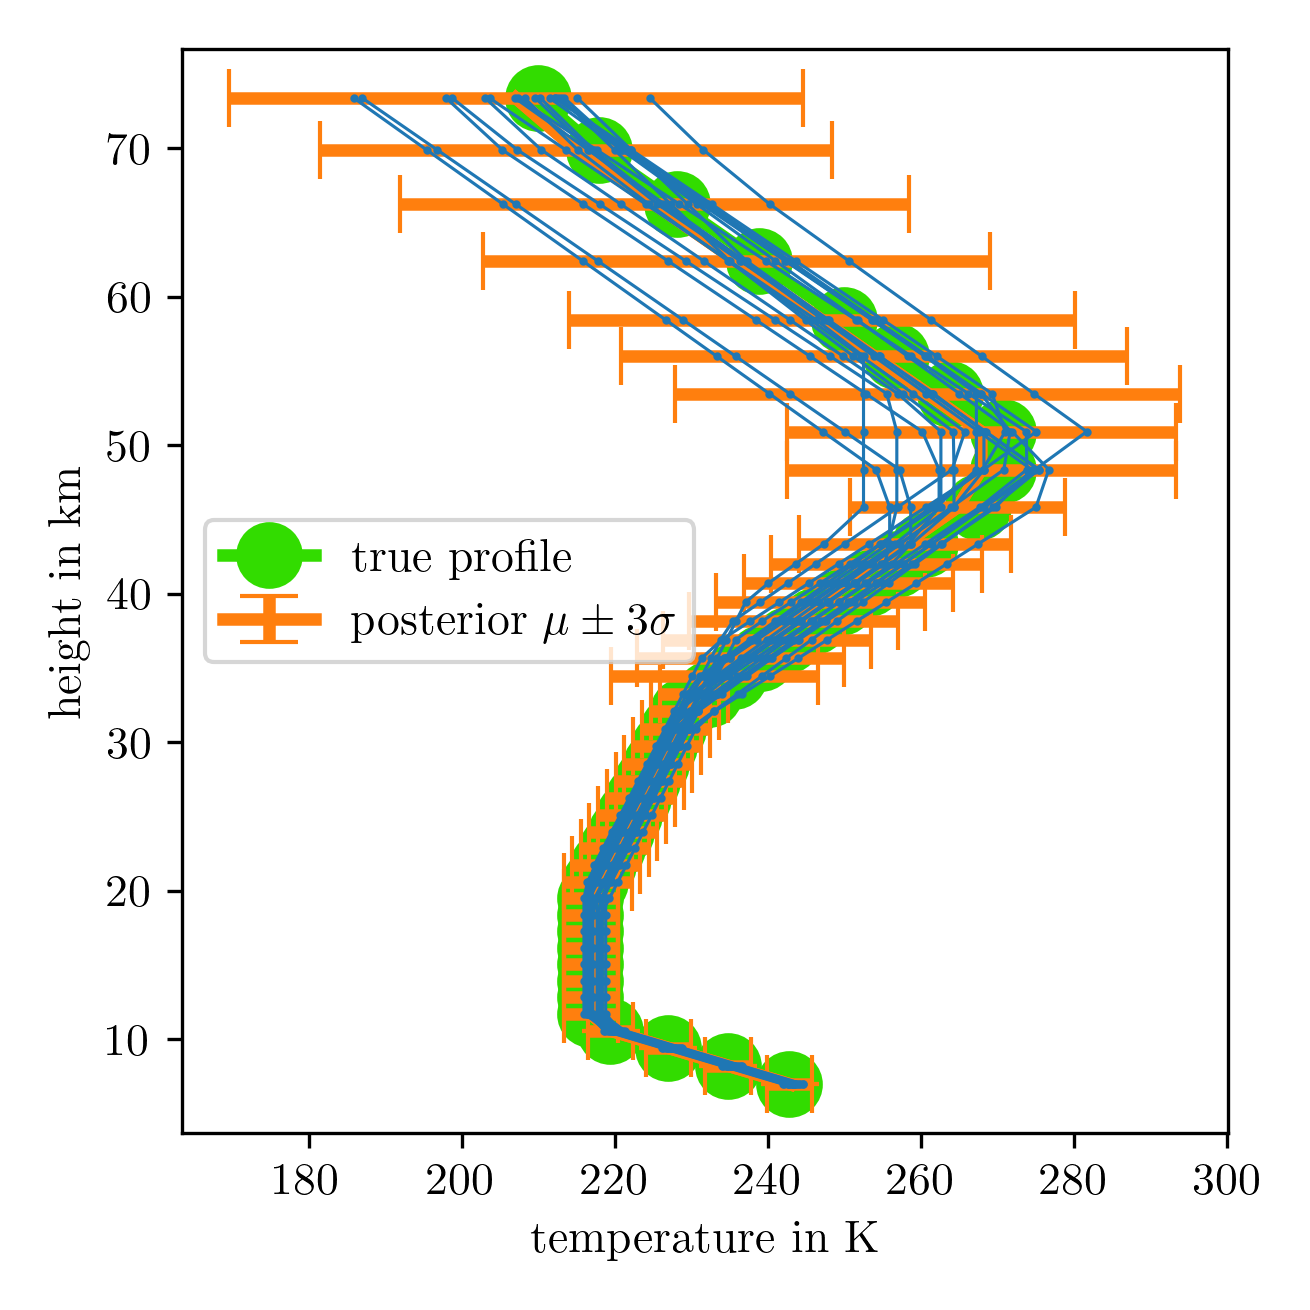
\includegraphics{TempPostMeanSigm.png} 
	\caption[Temperature posterior samples.]{Plot of posterior temperature profiles according to Eq.~\ref{eq:tempFunc} and hyper-parameter samples from the marginal posterior distribution $\pi(\bm{\theta},\lambda,\gamma  | \bm{y})$.}
	\label{fig:TempPost}
\end{figure}
\begin{figure}[ht!]
	\centering
	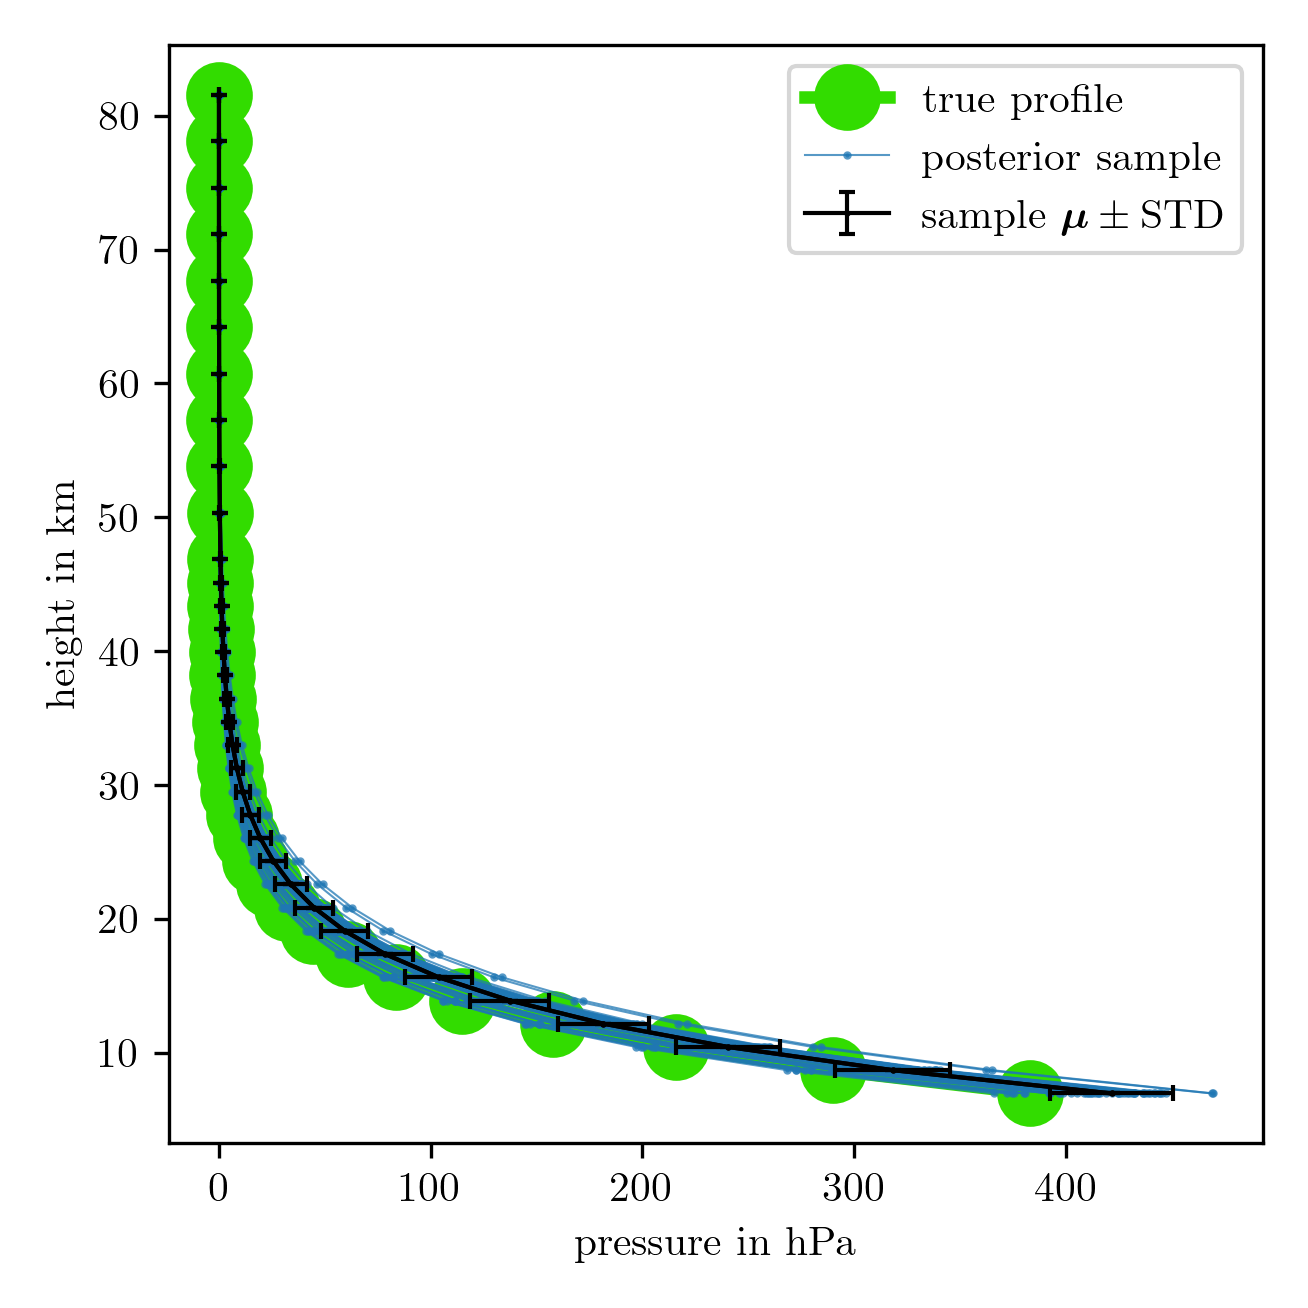
\includegraphics{PressPostMeanSigm.png}
	\caption[Pressure posterior samples.]{Plot of posterior pressure profiles according to Eq.~\ref{eq:pressFunc} and hyper-parameter samples from the marginal posterior distribution $\pi(\bm{\theta},\lambda,\gamma  | \bm{y})$.}
	\label{fig:PressPost}
\end{figure}
\clearpage

\subsection{Full Conditional Posterior -- Ozone}
Due to the large number of hyper-parameters calculating the posterior mean $\bm{\mu}_{\bm{x}|\bm{y}}$ and $\bm{\Sigma}_{\bm{x}|\bm{y}}$ covariance via quadrature as in Eq.~\ref{eq:MeanGenInt} and~\ref{eq:CoVarGenInt} is computationally not feasible.
If the full conditional posterior is a normal distribution, then the randomise then optimise (RTO) method provides a scheme to obtain an ozone sample from $\pi(\bm{x}|\bm{\theta}, \delta, \gamma, \bm{y})$ with $\delta = \lambda \, \gamma$.
We introduce the RTO method for general case first and then draw ozone samples from $\bm{x}^{(k)} \sim \pi(\bm{x}|\bm{\theta}^{(k)} , \delta^{(k)} , \gamma^{(k)} , \bm{y})$ conditioned on independent marginal posterior samples $\bm{\theta}^{(k)} , \delta^{(k)} , \gamma^{(k)} \sim \pi(\bm{\theta} , \delta , \gamma | \bm{y})$.


\subsubsection{Randomise then optimise}
\label{subsec:RTO} 
As in~\cite{bardsley2012mcmc} rewrite the full conditional posterior (see Eq.~\ref{eq:CondPostLin}) as
\begin{align}
	\pi(\bm{x} | \bm{\theta},  \delta, \gamma, \bm{y}) & \propto \pi(\bm{y}|\bm{x},  \bm{\theta}, \gamma) \pi(\bm{x}| \delta)\\
	&\propto \exp \left(-\frac{1}{2} (\bm{A}_{\bm{\theta}}  \bm{x} - \bm{y})^T \bm{\Sigma}^{-1}_{\gamma} (\bm{A}_{\bm{\theta}}   \bm{x} - \bm{y})\right) \exp \left(-\frac{1}{2} (\bm{\mu} - \bm{x} )^T \bm{Q}_{\delta}(\bm{\mu} - \bm{x} ) \right),\\
	& = \exp \left( - \frac{1}{2}\left\lVert \hat{\bm{A}} \bm{x} - \hat{\bm{y}} \right\rVert_{L^2}^2 \right),
\end{align}
where
\begin{align}
	\label{eq:minimizer}
	\hat{\bm{A}} \coloneqq 
	\begin{bmatrix}
		\bm{\Sigma}_{\gamma}^{-1/2} \bm{A}_{\bm{\theta}} \ \\
		\bm{Q}_{\delta}^{1/2}
	\end{bmatrix}, \quad 
	\hat{\bm{y}} \coloneqq 
	\begin{bmatrix}
		\bm{\Sigma}_{\gamma}^{-1/2} \bm{y} \\
		\bm{Q}_{\delta}^{1/2} \bm{\mu}
	\end{bmatrix} , 
\end{align}
$\bm{Q}_{\delta}$ is the prior precision, $\bm{\mu}$ the prior mean and $\bm{\Sigma}_{\gamma}$ the noise covariance (see also~\cite{bardsley2014randomize,BardsleyTC2019RTO}).
A sample $\bm{x}^{(k)}$ from the full conditional posterior $ \pi(\bm{x}|   \bm{\theta},  \delta, \gamma,  \bm{y})$ is obtained by minimising the following equation:
\begin{align}
	\bm{x}^{(k)} = \arg \min_{\bm{x}} \lVert \hat{\bm{A}} \bm{x} - ( \hat{\bm{y}} + \bm{b} ) \rVert_{L^2}^2 
\end{align}
with a random additive perturbation $\bm{b} \sim \mathcal{N}(\bm{0}, \bm{I})$.
Similar to Sec.~\ref{sec:reg}, this expression becomes
\begin{align}
	\label{eq:RTO}
	\left( \bm{A}_{\bm{\theta}}^T \bm{\Sigma}^{-1}_{\gamma} \bm{A}_{\bm{\theta}} + \bm{Q}_{\delta} \right) \bm{x}^{(k)} = \bm{A}_{\bm{\theta}}^T \bm{\Sigma}^{-1}_{\gamma} \bm{y} + \bm{Q}_{\delta} \bm{\mu} + \bm{v}_1 + \bm{v}_2,
\end{align}
%where the term $-\hat{\bm{A}}^T \bm{b}$ is decomposed as $\bm{v}_1 + \bm{v}_2$, 
with $\bm{v}_1 \sim \mathcal{N}(\bm{0}, \bm{A}_{\bm{\theta}}^T \bm{\Sigma}^{-1}_{\gamma} \bm{A}_{\bm{\theta}})$ and $\bm{v}_2 \sim \mathcal{N}(\bm{0}, \bm{Q}_{\delta})$, representing independent Gaussian random variables~\cite{bardsley2012mcmc, fox2016fast}.


\subsubsection{Posterior ozone samples}
More explicitly, conditioned on an independent $\bm{\theta}^{(k)},\lambda^{(k)},\gamma^{(k)} \sim \pi(\bm{\theta},\lambda,\gamma | \bm{y})$, one full conditional posterior sample is given as  
\begin{align}
	\label{eq:RTOAppl}
	\bm{x}^{(k)} = 	\Big(  \underbrace{\gamma^{(k)} \bm{A}_{\bm{\theta}^{(k)}}^T\bm{A}_{\bm{\theta}^{(k)}} +  \delta^{(k)}\bm{L}}_{\bm{B}^{(k)}} \Big)^{-1} \left(  \gamma^{(k)}  \bm{A}_{\bm{\theta}^{(k)}}^T\bm{y} +\sqrt{\gamma^{(k)}} \bm{A}_{\bm{\theta}^{(k)}}^T \tilde{\bm{v}}_1 + \sqrt{\delta^{(k)}}\bm{L}^{1/2}\tilde{\bm{v}}_2\right)
\end{align}
with $\tilde{\bm{v}}_1 \sim \mathcal{N}(\bm{0},  \bm{I})$, $\tilde{\bm{v}}_2 \sim \mathcal{N}(\bm{0}, \bm{I} )$, $\bm{Q}_{\delta} = \delta  \bm{L} $, $\bm{\Sigma}^{-1}_{\gamma} = \gamma \bm{I}$ and $\bm{L}^{1/2}$ is the Cholesky decomposition of $\bm{L}$ \cite{bardsley2012mcmc}.
Note that $\bm{v}_1 \in \mathbb{R}^m$ and $\bm{v}_2 \in \mathbb{R}^n$.
The Cholesky factorisation of $\bm{B}^{(k)}$ and $\bm{L}$ is obtained via the Python function \texttt{numpy.linalg.cholesky} and \texttt{scipy.linalg.cho\_solve} is used to solve for $\bm{x}^{(k)}$.
If calculating the Cholesky decomposition of $\bm{L}$ or constructing $\bm{L}$ is expensive and $\bm{L}$ can be represented as a sum over small $2\times2$ rank-1 matrices (see $\bm{L}$ in Eq.~\ref{eq:LaplRegTheo}), then a sample $\bm{v}_2 \sim \mathcal{N}(\bm{0}, \bm{Q}_{\delta})$ can be obtained by drawing $n$ random variables from $\mathcal{N}(0,1)$ without explicitly forming $\bm{L}$~\cite{fox2016fast}.

In Fig.~\ref{fig:O3Post}, 50 posterior ozone samples and a sample mean from 1000 full conditional posterior samples.
The posterior ozone mean is much smaller than the ground truth, especially around the ozone peak.
Compared to the posterior pressure in Fig.~\ref{fig:PressPost}, which is slightly larger than the ground truth, we can conclude that pressure and ozone are highly correlated.

Additionally, the individual posterior samples are more prior-dominated through larger $\lambda$ values (see Fig.~\ref{fig:PostHistTT0}) and hence smoother compared to the previously calculated ozone posterior profiles.
Again, we are not able to recover the second ozone peak at high altitudes.


\begin{figure}[ht!]
	\centering
	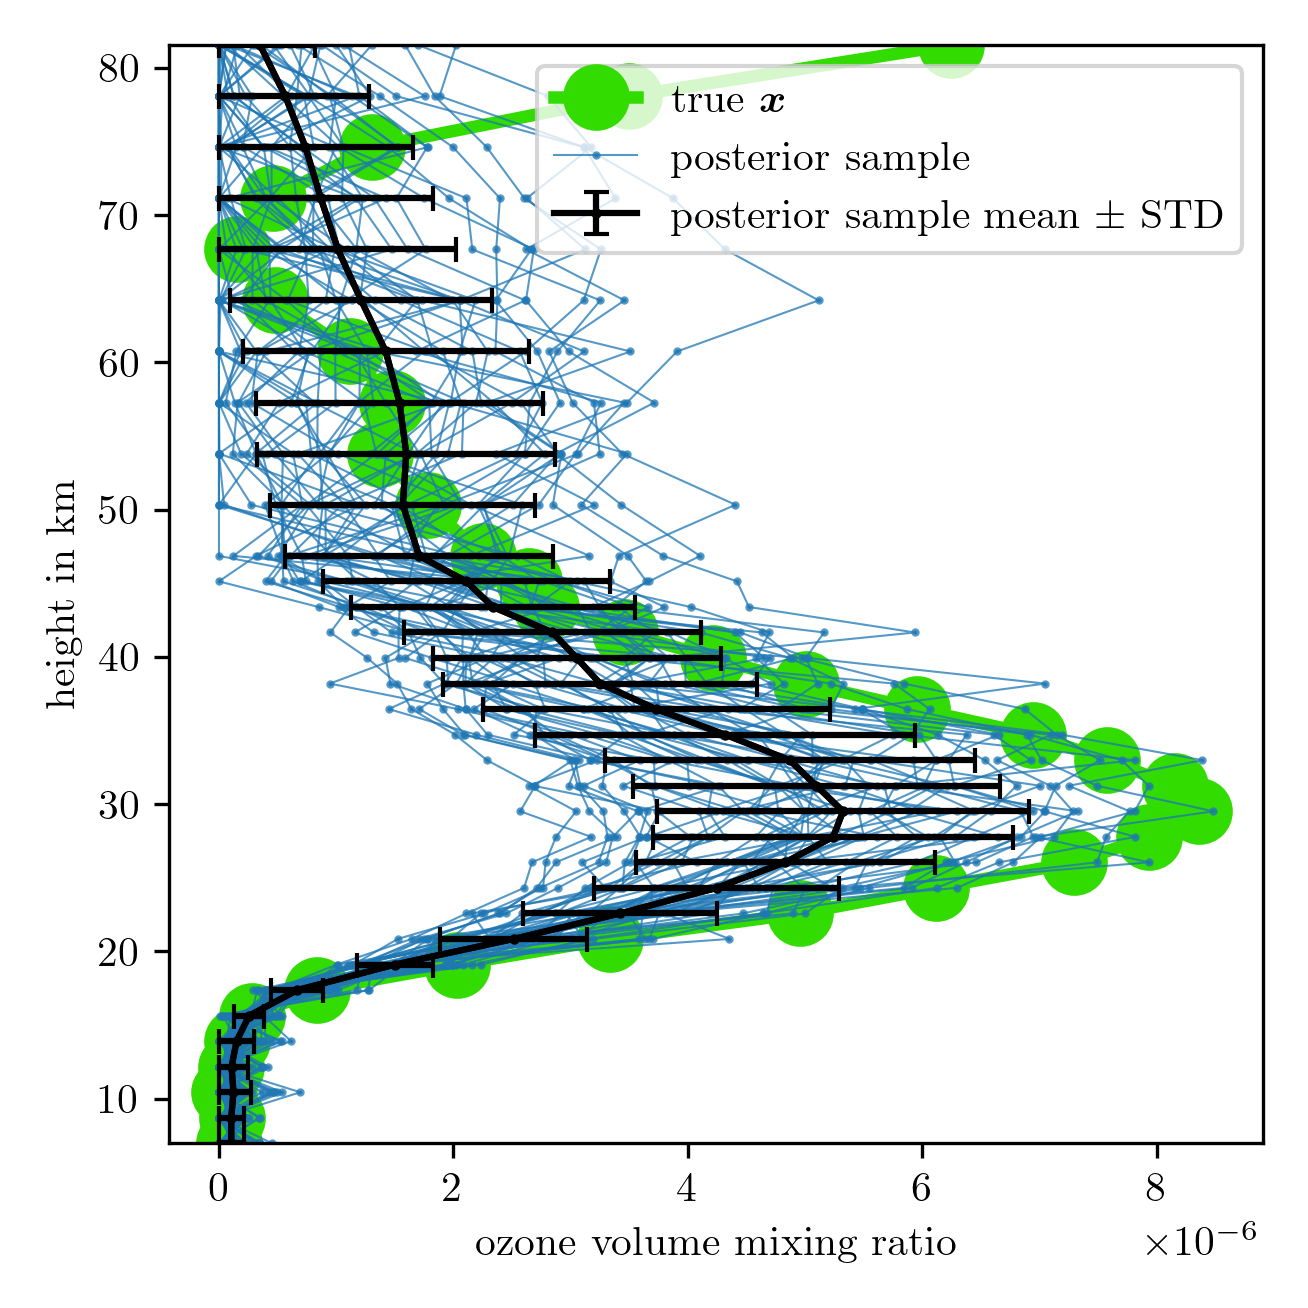
\includegraphics{FullO3Res.png}
	\caption[Pressure posterior samples.]{Plot of ozone samples from the full conditional posterior $\pi(\bm{x} | \bm{\theta},  \delta, \gamma, \bm{y})$ via the RTO method.}
	\label{fig:O3Post}
\end{figure}


\clearpage